%!TEX root = P231_notes.tex

\section{Linear Algebra Review}

As physicists, linear algebra is part of our \acro{DNA}, from the vector calculus in our first electrodynamics course to quantum mechanics. So why should we patronize ourselves with yet another review of linear algebra?
%
We want to understand Green’s functions the inverse of a matrix. The `matrix' in question is the differential operator $\mathcal O$ in \eqref{eq:greens:function:equation}.
%
This is important:
\begin{align}
	\text{differential operator}
	&=
	\infty\text{-dimensional matrix} \ .
\end{align}
If differential operators are matrices, what vector space do these matrices act on? These matrices act on a space of functions, which turns out to be a vector space:
\begin{align}
  \text{function space} &= \infty\text{-dimensional vector space} \ .
\end{align}
Don't be intimidated by terminology like \emph{function space}; this is just an abstract place where functions live. Just recall back to your intuition from \acronum{3D} Euclidean vector space, $\mathbb{R}^3$: any 3-vector $\vec{v}$ lives in the vector space $\mathbb{R}^3$. If we transform $\vec{v}$ by a linear transformation ${A}$, you get a new vector  $\vec{w} = {A}\vec{v} \in \mathbb{R}^3$ that is also in the vector space.

%
Weird things can happen when we extend our intuition from finite things to infinite things\footnote{For example, the Hilbert Hotel puzzle.}, but for this course we'll try to draw as much intuition as we can from finite dimensional linear algebra to apply it to infinite dimensional function spaces.

\subsection{The basics}

A \textbf{linear transformation} $A$ acts on a vector $\vec{v}$ as $A\vec{v}$. 
This transformation satisfies
\begin{align}
  A(\alpha \vec{v}+ \beta \vec{w}) = \alpha A\vec{v} + \beta A\vec{w} \ .
\end{align}
Here $\alpha$ and $\beta$ are numbers.
%
This is conventionally matrix multiplication. The result is also a vector. One way that we like to think about vectors is as columns of elements:
\begin{align}
  \begin{pmatrix}
    v^{1} \\ v^{2} \\ \vdots \\ v^{N}
  \end{pmatrix} \ ,
  \label{eq:vector:def:as:column}
\end{align}
where $N$ is the \textbf{dimension} of the vector space. Our notation is that $v^i$ refers to the $i^\text{th}$ component of $\vec{v}$. Sometimes---as physicists---we refer to $v^i$ as the vector itself, which is a slight abuse of notation that occasionally causes confusion.

In this course we always assume a nice orthonormal basis. In this case, $(\vec{v} + \vec{w})^i = v^i + w^i$.
\begin{exercise}
Convince yourself that adding vectors becomes more complicated in polar coordinates. Namely, $(\vec{v} + \vec{w})^i \neq v^i + w^i$.
\end{exercise}

Because the linear transformation of a vector is another vector, we know that the sequential application of linear transformations is itself a linear transformation. This is a bombastic way of saying that you can multiply matrices to produce a matrix.  Here’s how it works in two dimensions. A transformation that takes vectors into vectors takes the following form:
\begin{align}
  A &= 
  \begin{pmatrix}
   A^{1}_{\phantom{1}1} & A^{1}_{\phantom{1}2}
   \\
   A^{2}_{\phantom{1}1} & A^{2}_{\phantom{1}2}
  \end{pmatrix} \ .
\end{align}
We have introduced upper and lower indices; for now treat this as a definition. This sometimes causes confusion. So here are some guidelines:
\begin{itemize}
	\item Treat the upper and lower indices as a definition. The components of the linear transformation $A$ are \emph{defined} by $A^i_{\phantom{i}j}$ where $i$ is the row number and $j$ is the column number. 
	\item We have not yet explained the significance of the heights, but for now we mandate that the first index is always upper and the lower index is always lower. The following objects do not (yet) make sense: $A^{1}_{\phantom{1}2}$ and \emph{not} $A_{12}$, $A^{12}$, or $A_{1}^{\phantom{1}2}$.
	\item We will soon define \emph{additional machinery} to raise and lower indices shortly. This is takes us from a vector space to a metric space.
	\item The heights of the indices are a convenient shorthand notation that we will elucidate shortly; it is related to the choice of upper indices in \eqref{eq:vector:def:as:column}.
	\item All of this may be familiar from special relativity. Extra credit if you realize that this should also be familiar from quantum mechanics.
\end{itemize}
If you’re squeamish about the indices, don’t worry: the elements of $A$ have two indices, the first one is written a little higher than the second one. This notation is neither mathematics nor physics, it’s a convention that we use for future convenience.

The action of a linear transformation $A$ on a vector $\vec{v}$ is:
\begin{align}
  A\vec{v}
  =
  \begin{pmatrix}
    A^{1}_{\phantom{1}1} & A^{1}_{\phantom{1}2}
   \\
   A^{2}_{\phantom{2}1} & A^{2}_{\phantom{2}2}   
  \end{pmatrix} 
  \begin{pmatrix}
    v^1\\
    v^2
  \end{pmatrix}
  =
  \begin{pmatrix}
    A^1_{\phantom{1}1} v^1 + A^1_{\phantom{1}2}v^2\\
    A^2_{\phantom{2}1} v^1 + A^2_{\phantom{2}2}v^2
  \end{pmatrix} \ .
\end{align}
Look at this carefully. The components of the new vector $(A \vec{v})^i$ are sums. In each term, the second/lower index of an $A$ element multiplies the component of $\vec{v}$ with the same index. The first/upper index of $A$ tells you whether that term should is in $(A \vec{v})^1$ or $(A \vec{v})^2$. 

A generic component of $(A\vec{v})$ is
\begin{align}
  (A\vec{v})^i = \sum_j A^i_{\phantom{i}j} v^j
  = A^i_{\phantom{i}j} v^j \quad \text{(Einstein convention)}
   \ .
\end{align}
On the right-hand side we use Einstein notation: \emph{we implicitly sum over repeated upper/lower indices}. We will use this notation from now on.
%
If you are at all in doubt about this, please work out the $2\times 2$ case carefully and compare to the succinct notation above. 

\begin{exercise}
Consider three-dimensional Euclidean space, $\mathbb{R}^3$. A linear transformation $A$ on this space is a $3\times 3$ matrix with elements of the form $A^i_{\phantom{i}j}$. Explicitly write out the second component of the vector $A\vec{v}$. This is a sum of three terms.
\end{exercise}

If $A$ and $B$ are linear transformations, then $A+B$ is a linear transformation. The components of $A+B$ are simply the piecewise sum of the corresponding components of $A$ and $B$:
\begin{align}
  (A+B)^i_{\phantom i j} = A^i_{\phantom i j} + B ^i_{\phantom i j} \ .
\end{align}


\subsection{Linear Transformations and Vector Spaces}

Let’s be a little more pedantic. We need to move past the idea that a vector $\vec{v}$ is some \emph{column of numbers}. A vector space is abstract and we need to to start thinking of vector spaces more generally. The layer of abstraction is encoded in the basis vectors, which we write as $\vec{e}_{(i)}$. For a space of dimension $N$, there are $N$ such vectors indexed by the subscript. Let us more formally write the vector $\vec{v}$ as
\begin{align}
  \vec{v} = 
  v^1 \vec{e}_{(1)}
  +
  v^2 \vec{e}_{(2)} + \cdots
  = v^i \vec{e}_{(i)} \ .
  \label{eq:v:v1:v2:v3}
\end{align}
These basis vectors may be unit vectors in space. In the `column of numbers' representation, they can be unit column vectors, e.g.
\begin{align}
  \vec{e}_{(1)}
  &= 
  \begin{pmatrix}
  1 \\ 0 \\ 0
  \end{pmatrix}
  &
    \vec{e}_{(2)}
  &= 
  \begin{pmatrix}
  0 \\ 1 \\ 0
  \end{pmatrix}
  &
  \cdots \ .
\end{align}
With this basis, \eqref{eq:v:v1:v2:v3} gives \eqref{eq:vector:def:as:column}
But these may be more general objects. For example, you can specify a color of light by specifying the red/green/blue content. We could have $\vec{e}_{(1)}$ be a unit amount of red light, $\vec{e}_{(2)}$ be a unit amount of green light, and $\vec{e}_{(3)}$ be a unit amount of blue light. Then a 3-vector $\vec{v}$ would correspond to light of a particular color. This color space is a vector space.




\subsection{A funny vector space: histogram space}
\label{sec:histogramspace}

Here’s a funny vector space that we’re going to use as a pedagogical crutch. Imagine histogram-space. The basis vectors are:

\begin{center}
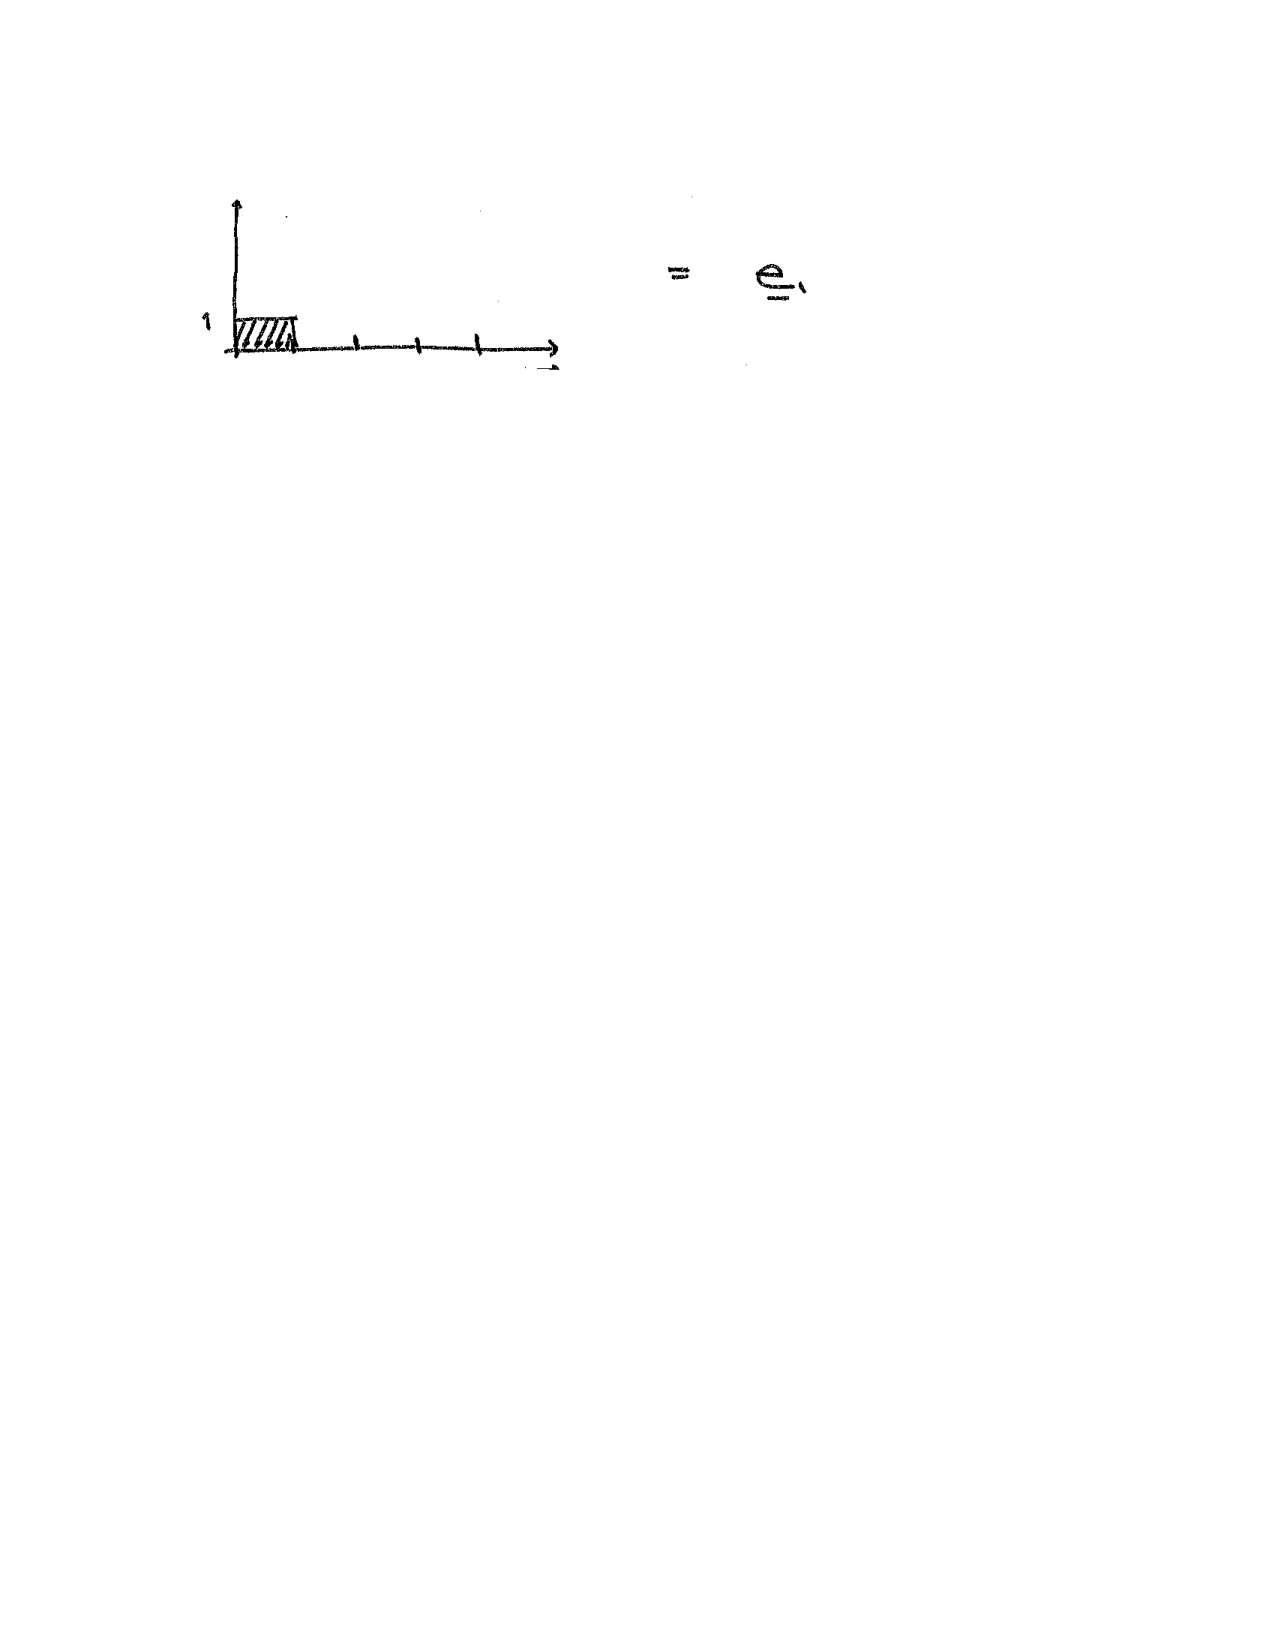
\includegraphics[width=.45\textwidth]{figures/lec02_e1.pdf}
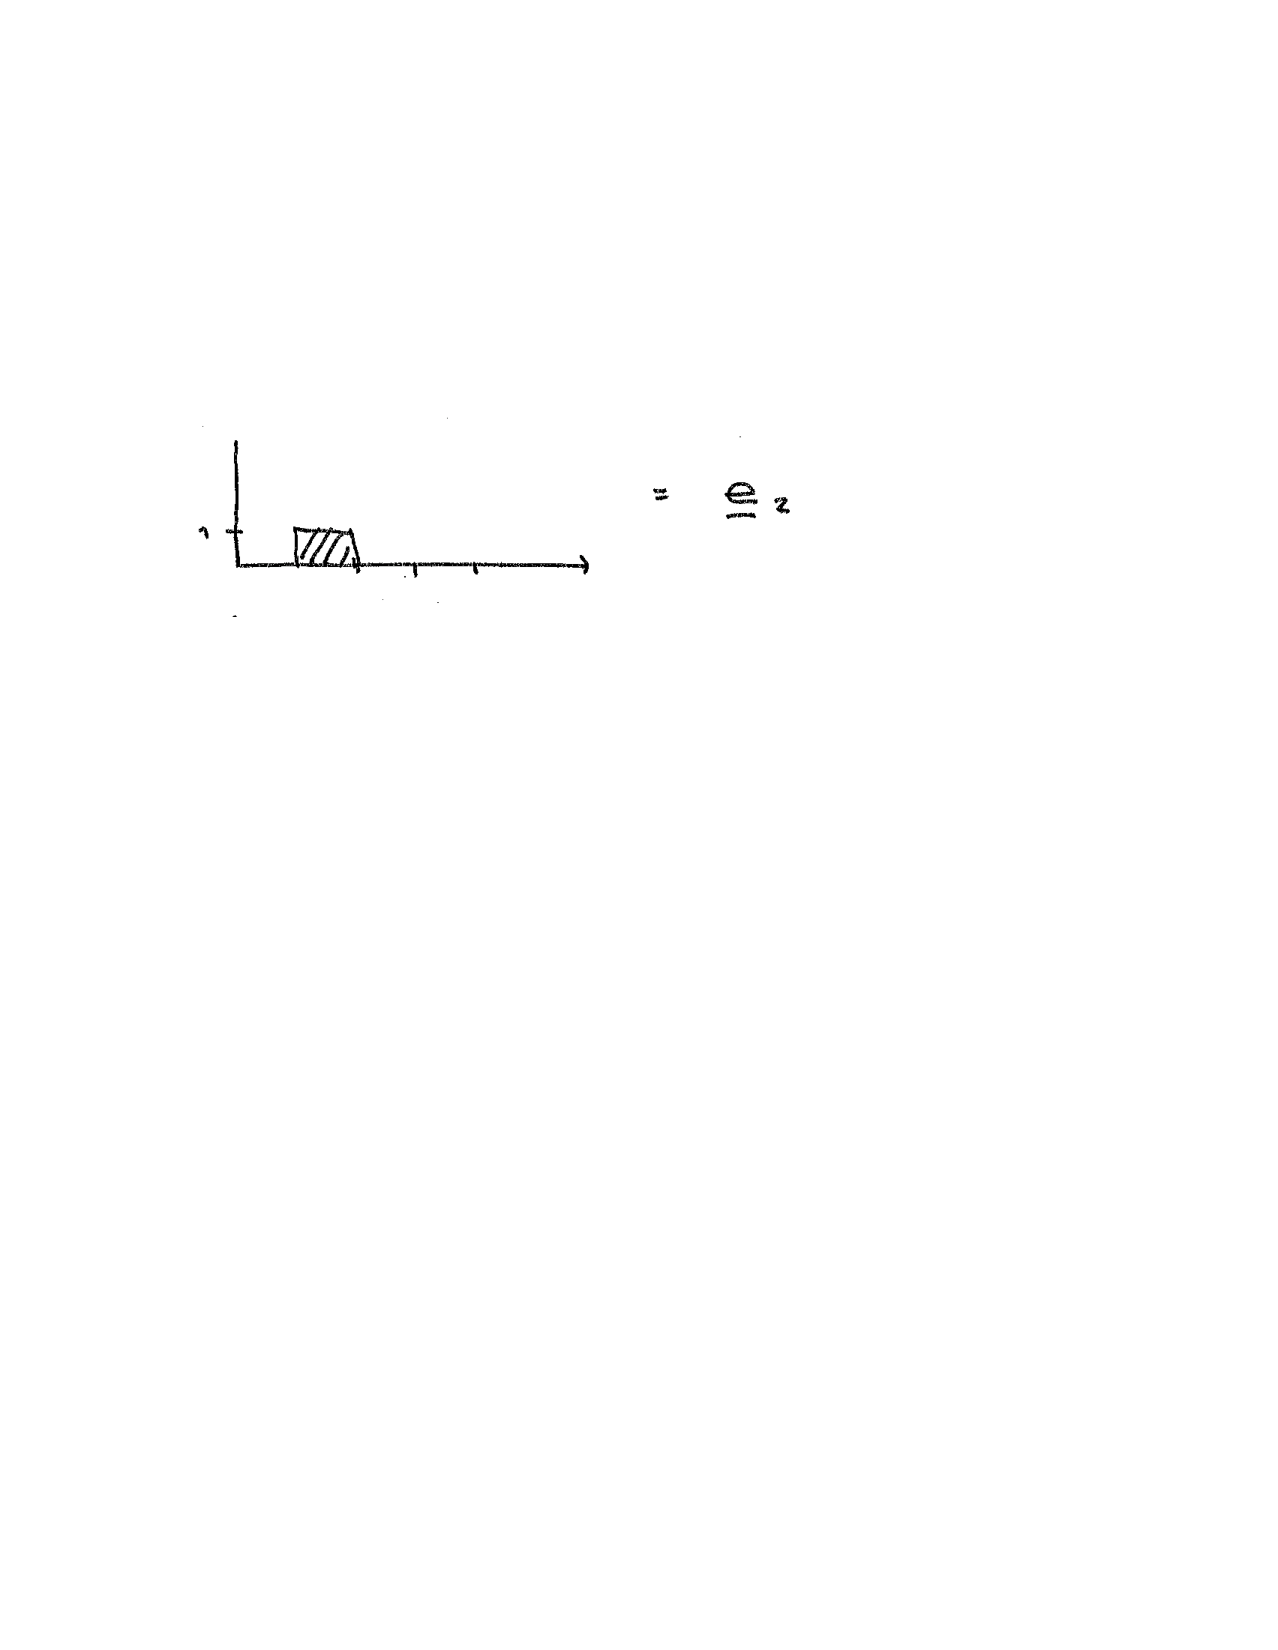
\includegraphics[width=.45\textwidth]{figures/lec02_e2.pdf}\\
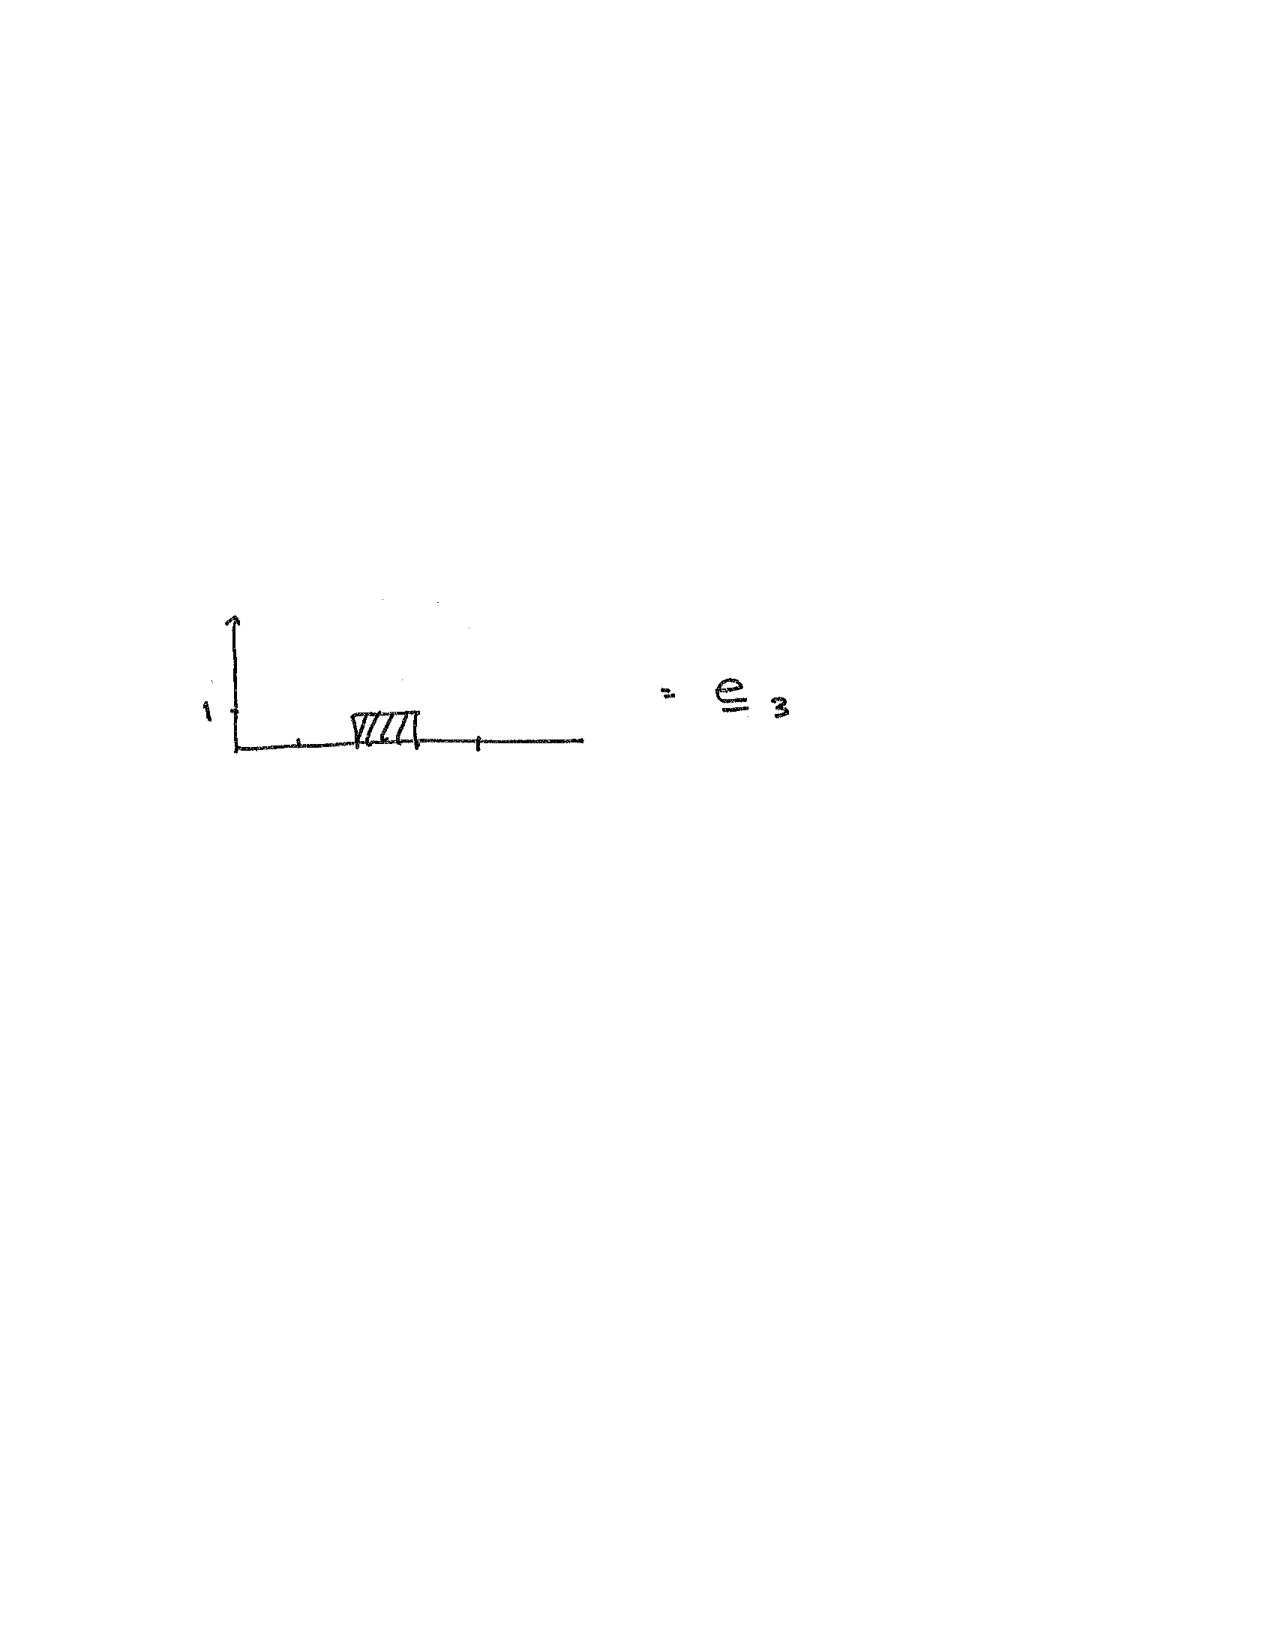
\includegraphics[width=.45\textwidth]{figures/lec02_e3.pdf}
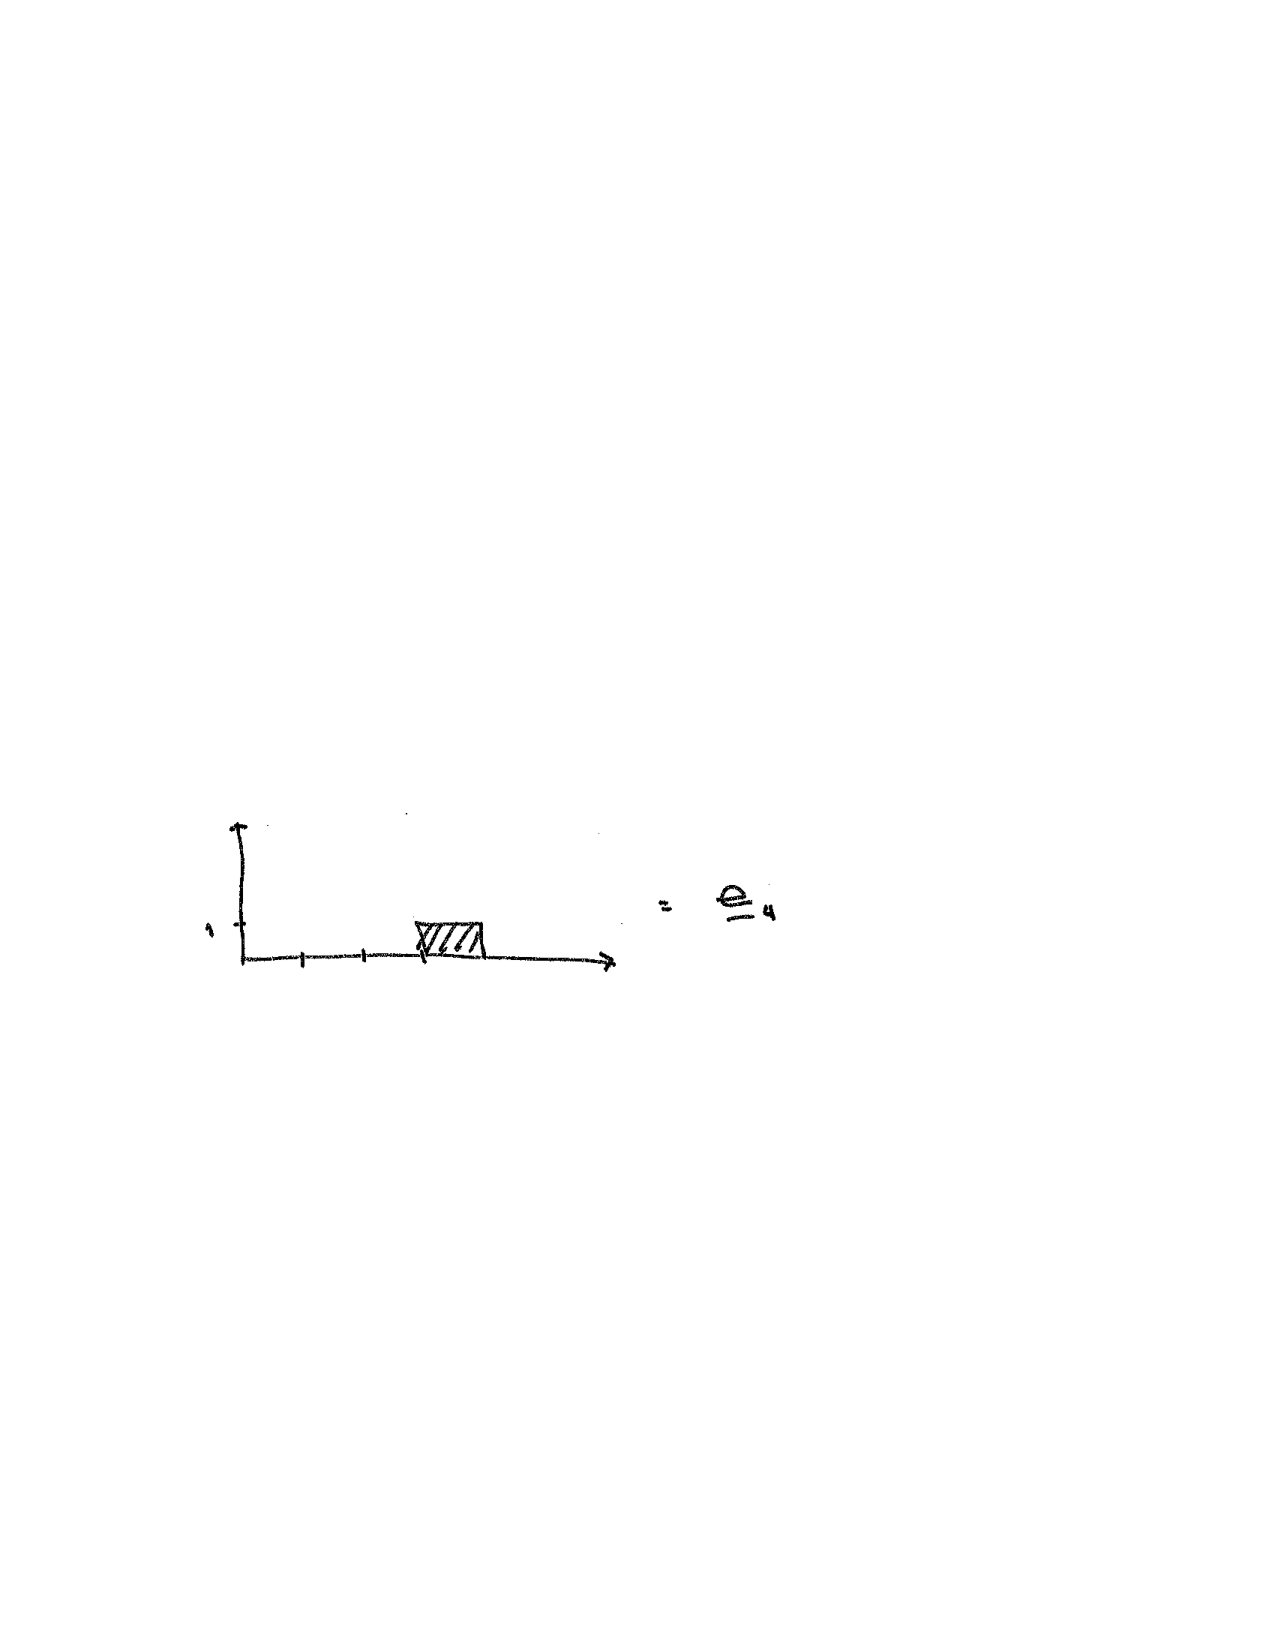
\includegraphics[width=.45\textwidth]{figures/lec02_e4.pdf}
\end{center}

\noindent This is a basis for a histogram over unit bins from $x=0$ to $x=4$. A vector in this space is, for example:

\begin{center}
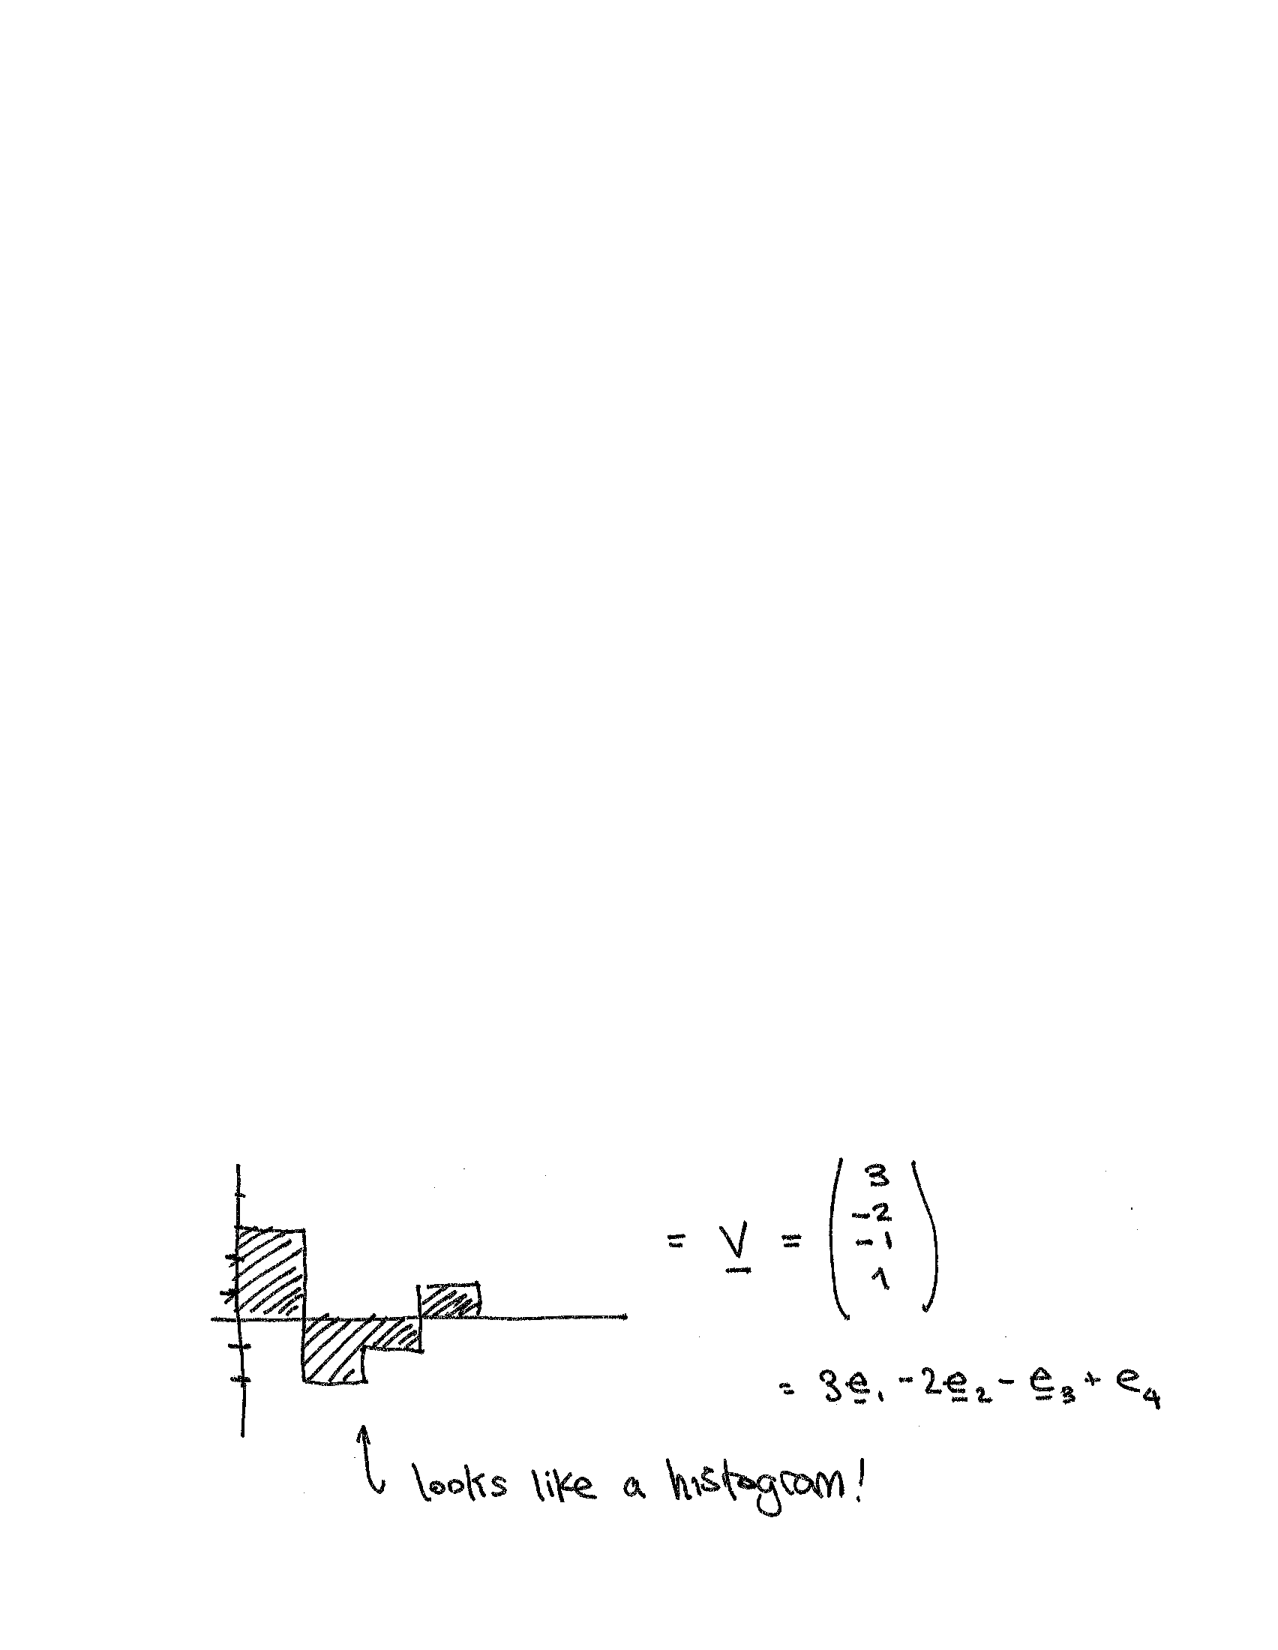
\includegraphics[width=.8\textwidth]{figures/lec02_hist.pdf}
\end{center}

\noindent We can perform a linear transformation $A$ on $\vec{v}$ which outputs another vector. Let’s say it’s this:


\begin{center}
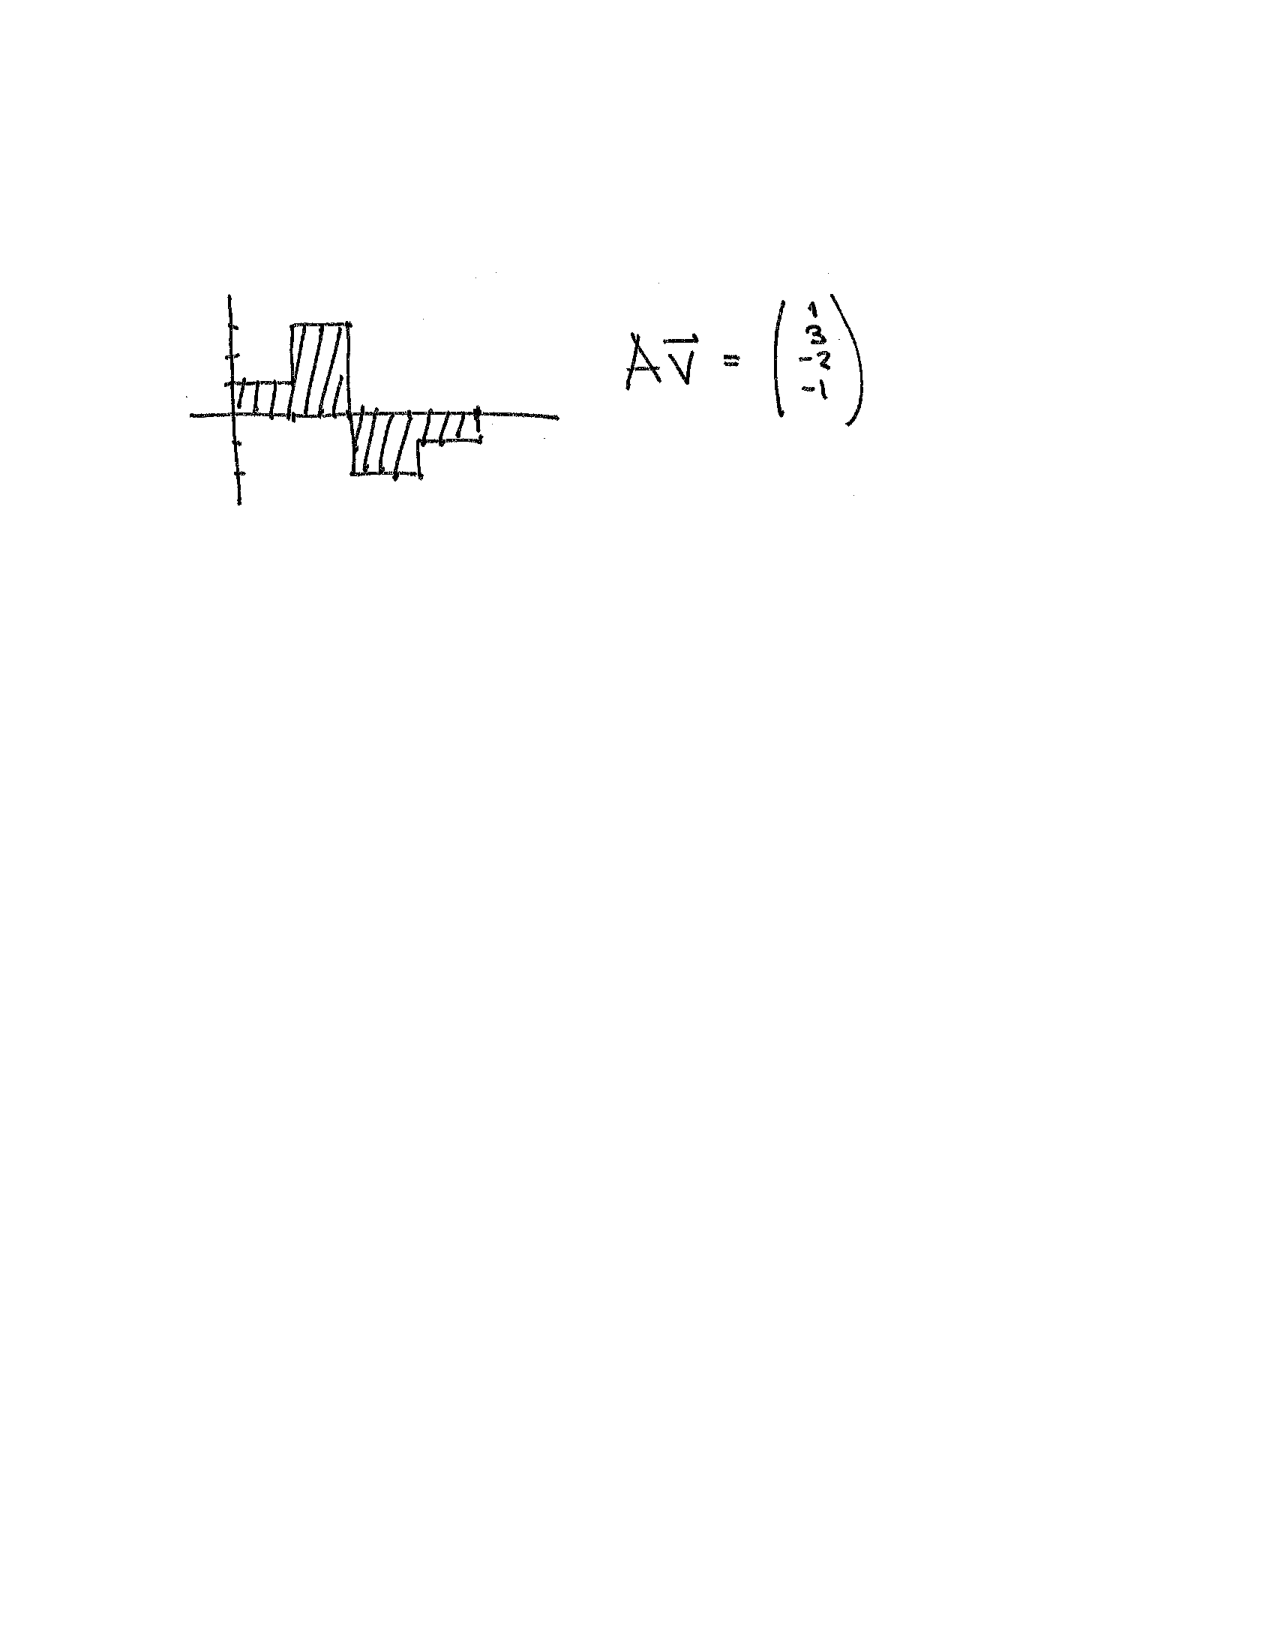
\includegraphics[width=.8\textwidth]{figures/lec02_hist2.pdf}
\end{center}

\begin{exercise}
From the image above, can you derive what $A$ is? 
\end{exercise}

\noindent The answer to the above exercise is \emph{no}. Please make sure you convince yourself why: there are many different transformations that convert to old histogram into the new histogram. If you're not convinced: the matrix $A$ is $4\times 4$ and thus has 16 entries that we need to define. The matrix equation $A\vec{v} = \vec{w}$ for known vectors $\vec{v}$ and $\vec{w}$ encodes only four equations.

The power of this admittedly strange formalism is that we can think of these histograms as approximations of continuous functions:

\begin{center}
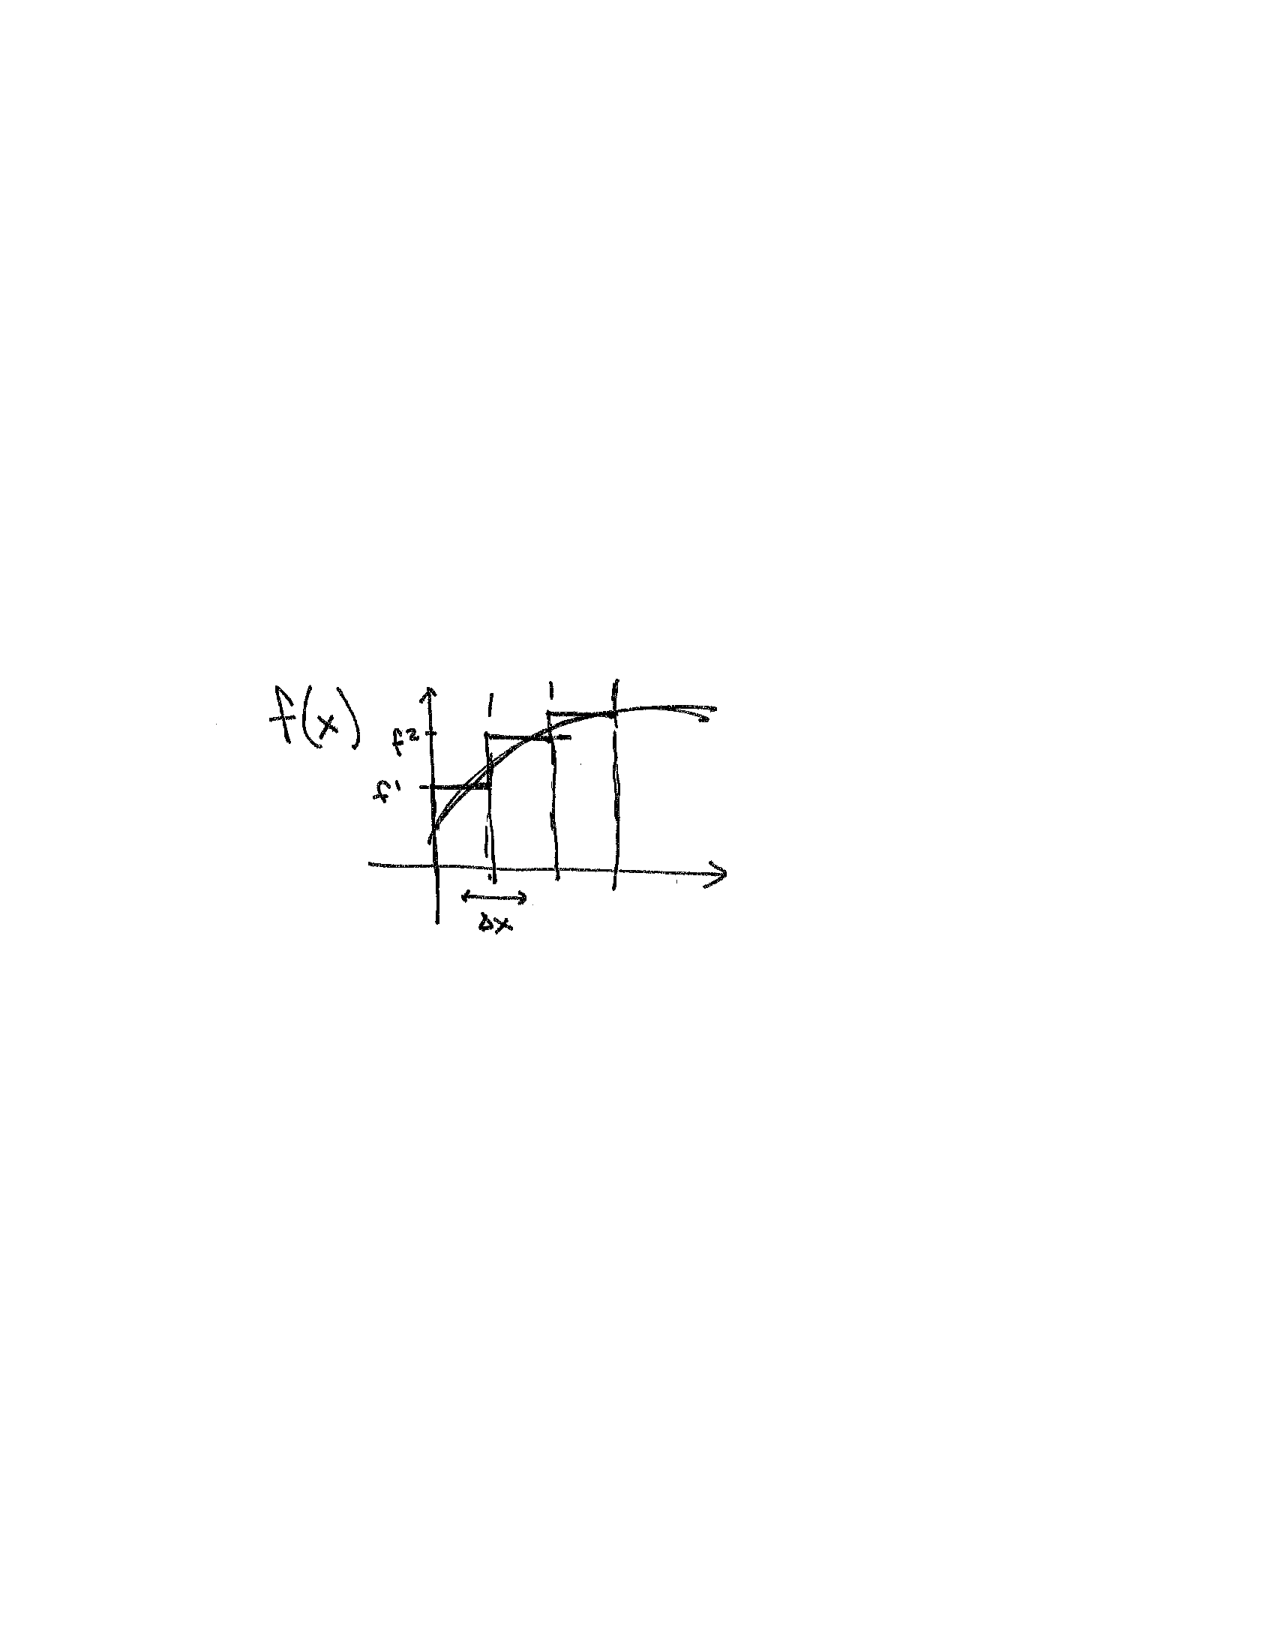
\includegraphics[width=.4\textwidth]{figures/lec02_histfun.pdf}
\end{center}

Thus a vector in this approximate (discretized) \emph{function} space is 
\begin{align}
  \vec{f} = 
  \begin{pmatrix}
    f^1 \\
    f^2 \\
    \vdots\\
    f^N
  \end{pmatrix} \ .
\end{align}

\subsection{Derivative Operators}

Our discretized function space allows us to define a [forward] derivative\footnote{One could have also defined a backward derivative where $(f')^i \sim f^{i}-f^{i-1}$ \ . Note that you \emph{cannot} try to make this symmetric by defining a `centered' derivative like $(f')^i \sim f^{i+1/2}-f^{i-1/2}$ because there's no such thing as a fractional index. If you tried to write $(f')^i\sim f^{i+1}-f^{i-1}$ you're making a worse approximation. If you're like me, the fact that there's some asymmetry in how we define the first derivative is deeply unsettling. There's something to this intuition!}:
\begin{align}
  \vec{f'} =
  \frac{1}{\Delta x}
  \begin{pmatrix}
    f^2 - f^1 \\
    f^3 - f^2 \\
    \vdots
    \\
    f^{i+1}-f^i
    \\
    \vdots
  \end{pmatrix} \ .
\end{align}
This is familiar if you’ve ever had to manually program a derivative into a computer program. Note that the right-hand side looks like a linear transformation of $\vec{f}$. In other words, we expect to be able to write a matrix $D$ so that
\begin{align}
  \vec{f'} = D\vec{f} \ .
\end{align}
One problem is apparent: what happens at the `bottom’ of the vector? What is the last component of the derivative, $\vec{f'}^N$? Formally, this is
\begin{align}
  {(f')}^N = \frac{1}{\Delta x}(f^{N+1} - f^N) \,
\end{align}
but now we have no idea what $f^{N+1}$ is. That was never a component in our vector space. There is no $\vec{e}_{(N+1)}$ basis vector. 
%
This demonstrates and important lesson that we’ll need when we move more formally to function spaces:
\begin{quote}
\textbf{Boundary conditions are part of the definition of the function space}.   
\end{quote}
That was so important that I put the whole damn sentence in boldface and set it in the middle of the line. The significance of boundary conditions may be a bit surprising---but think of this as part of the definition of which functions we allow into our function space. 
%
\begin{example}
When one first learns about Fourier series with Dirichlet boundary conditions, one finds that the Fourier expansion \emph{only} contains sines. The solution to the wave equation in such a system is some function that is zero at each endpoint. So the function space relevant to the system is composed only of functions that are zero at each endpoint.
\end{example}
%
For now let’s assume \textbf{Dirichlet boundary conditions}. A convenient way to impose this is to define what happens to all functions outside the domain of the function space:
\begin{align}
  f^{i > N} = f^{i < 1} = 0 \ .
\end{align}
This solves the problem of the derivative on the last component:
\begin{align}
  {(f')}^N = \frac{1}{\Delta x}(f^{N+1} - f^N) 
  = 
  \frac{- f^N}{\Delta x}  \ .
\end{align}
Alternatively, we could have also imposed \textbf{periodic boundary conditions}:
\begin{align}
  f^{i} &= f^{i+ kN}
  & k\in \mathbb{Z} \ .
\end{align}
This would then give
\begin{align}
  {(f')}^N = \frac{1}{\Delta x}(f^{N+1} - f^N) 
  = 
  \frac{1}{\Delta x}(f^{1} - f^N) 
  \ .
\end{align}
Periodic boundary conditions amount to wrapping the $x$-axis into a circle. Older folks sometimes call this \emph{Asteroids} boundary conditions. I'd also accept \emph{Star Control} boundary conditions. Periodic boundary conditions show up \emph{all} the time in physics. Sometimes they show up in obvious places, like the Brillouin zone of a crystal lattice. Other times they show up in not-so-obvious places like the boundary conditions of the known universe. In addition to being crucial for a well-defined function space, the boundary conditions of a system establish its topology\footnote{I cannot over-emphasize the importance of topology in contemporary physics. Most of the physics you will learn in your first year graduate courses are intrinsically \emph{local} because the laws of physics are causal. Topological quantities are \emph{global}, they are integrals over an entire space. Because winding numbers (and their higher-dimensional cousins) are quantized, they are robust against perturbations. The number of holes in a donut is one, whether or not it's been slightly squished in the box. By the way, the best donuts in Southern California are from \emph{Sidecar Doughnuts} in Costa Mesa. Get the Basil Eggs Benedict donut before 11am; you can thank me later.}.

\begin{exercise}
We don't know anything about the universe outside the Hubble radius. Why do you think it would be reasonable in a physical model to \emph{assume} that it has periodic boundary conditions? Hint: what would happen to the $x$-momentum of an asteroid in the classic arcade game \emph{Asteroids} if the game did not have periodic boundary conditions? 
\end{exercise}

The second derivative may be defined symmetrically:
\begin{align}
  (f'')^i = \frac{(f^{i+1} - f^i) - (f^i - f^{i-1})}{\Delta x^2} \ .
\end{align}
You may pontificate about the reason why the first derivative does have a symmetric discretization while the second derivative does. 


\subsection{Derivatives in other function space bases}
\label{sec:derivatives}

There are other ways to write a discrete basis of functions. Here’s a natural one for functions that are up to second-order polynomials:
\begin{align}
  \vec{e}_{(0)} &= 1
  &
  \vec{e}_{(1)} &= x
  &
  \vec{e}_{(2)} &= x^2 \ .
\end{align}
Let’s sidestep questions about orthonormality for the moment. Clearly linear combinations of these basis functions can produce any quadratic function:
\begin{align}
  f(x) &= a x^2 + bx + c
  & \Rightarrow&&
  \vec{f} &=
  \begin{pmatrix}
     c \\ b \\ a
   \end{pmatrix} \ . 
\end{align}
The derivative operator has an easy representation in this space:
\begin{align}
  D = 
  \begin{pmatrix}
    0 & 1 & 0   \\
    0 & 0 & 2   \\
    0 & 0 & 0   
  \end{pmatrix} \ .
\end{align}
We can see that
\begin{align}
  D \vec{f}  &= 
  \begin{pmatrix}
     b \\
     2 a \\
     0
  \end{pmatrix} 
  &
  D^2 \vec{f}  &= 
  \begin{pmatrix}
     2a \\
     0 \\
     0
  \end{pmatrix} 
  &
  D^3 \vec{f}  &= 
  0 \ .
\end{align}
The last line is, of course, the realization that the third-derivative of a quadratic function vanishes. Feel free to attach mathy words to this like \emph{kernel}.

There are other bases that we may use for function space. A particularly nice one that we will use over and over is the Fourier basis, which we usually refer to as \emph{momentum space}. The basis vectors are things like sines, cosines, or oscillating exponentials. These do not vanish for any power of $D$.


\subsection{Locality}

Notice that in the histogram basis, the derivative matrix $D$ is sparse: it is zero everywhere away from the diagonal. The only non-zero elements on the $i^\text{th}$ row are around the $(i\pm 1)^\text{th}$ column.  Higher powers of $D$ sample further away, but the non-zero elements are always clustered near the diagonal.

This is simply a notion of \textbf{locality}. Remember the Taylor expansion:
\begin{align}
  f(x) = f(0) + f'(0) x + \frac{1}{2} f''(0)x^2 + \cdots \ .
\end{align}
If we think about the histogram as a discretization of a continuous function, then it is clear what the higher derivatives are doing. Given a function $f(x) = \vec{f}$, one might like to know about the function around some point $x_0$ corresponding to some index $i$. That is: $f^i = f(x_0)$. If you’d like to learn more about the function around that point, one can express the derivative at $x_0$. Thus $D\vec{f}$ says something about the slow, $D^2\vec{f}$ says something about the curvature, and so on. Because each successive power of $D$ samples terms further away from $f^i$, you can tell that these higher order terms are learning about the function further and further away from $x_0$. 

Now think about the types of differential equations that you’ve encountered in physics. They often include one or two derivatives. You hardly ever see three, four, or more derivatives\footnote{With some thought, it may also be clear why spatial derivatives typically appear squared.}. There’s a reason for this: at the scales that we can access experimentally, nature appears to be local. Our mathematical models of nature typically have locality built in\footnote{A recent counterexample: \url{https://www.quantamagazine.org/physicists-discover-geometry-underlying-particle-physics-20130917/}}. Physics at one spacetime point should not depend on spacetime points that are far away. 

This may be familiar from the idea of causality---the idea that $A$ \emph{causes} $B$ therefore $A$ must have happened \emph{before} $B$. One of the key results in special relativity is that causality can be tricky if two events do not occur at the same spacetime point. More carefully, $A$ can only cause $B$ if there is a timelike separation of the appropriate sign.  If we want to build causal theories of nature, then the dynamics at $x_0$ should not rely on what is happening at $x_1$, a finite distance away.\footnote{This is different from saying that information cannot propagate from $x_0$ to $x_1$; such propagation could come from some causal excitation of the electromagnetic field traveling every infinitesimal distance between the two positions. This is reminiscent of the classical Zeno's paradox.}


 

\subsection{Row Vectors and all that}

In high school we did not distinguish between row vectors and column vectors. They both seemed to convey the same information---they were simply one-dimensional arrays of numbers. Row vectors are just `tipped over.’ Such a tipping-over is convenient since you could apply the elementary schools rules of `matrix multiplication' have the row vector act on a column vector:
\begin{align}
  \begin{pmatrix}
    w_1 & w_2 & \cdots
  \end{pmatrix}
  \begin{pmatrix}
    v^1 \\
    v^2 \\
    \vdots
  \end{pmatrix}
  &= 
  w_1 v^1 + w_2 v^2 + \cdots \ .
\end{align}
In fact, this is like $\vec{w}^T$ is a function that acts \emph{linearly} on its argument, $\vec{v}$: 
\begin{align}
  \vec{w}^T(\vec v) &= w_1 v^1 + w_2 v^2 + \cdots \ .
  \label{eq:oneform:eats:vector}
\end{align}
Perhaps you see why we wrote the row vector components with lower indices, $w_i$ so that we may use Einstein summation notation: $\vec{w}^T\vec{v} = w_iv^i$.

Indeed, let is be a bit more formal about this. This layer of formalism is uncharacteristic of our approach in this course, but this underpins so much of the mathematical structure of our physical theories that it is worth getting right from the beginning. 
%
Let $V$ be a vector space. It contains vectors, $\vec{v}$. Sometimes these are called contravariant vectors or kets. They have basis vectors $\vec{e}_{(i)}$. 

Now introduce a related but \emph{completely distinct} vector space called $V^*$. This is the space of \textbf{dual vectors} to $V$. A \textbf{dual vector} is what you may know as a \textbf{row vector}, a \textbf{ket}, a \textbf{covariant vector}, or a [differential] \textbf{one-form}. These are all words for the \emph{same idea}. A dual vector, say $(\vec{w}^T)$ is a \emph{linear function that takes vectors and spits out numbers}:
\begin{align}
  \vec{w}^T \in V^* \Rightarrow \vec{w}^T: V \to \mathbb{R} \ .
 \end{align}
Don’t think about $\vec{w}^T$ as some kind of operation on a vector $\vec{w}\in V$; at least not yet. For now the `$^T$' is just part of the name of $\vec{w}^T$. The two spaces $V$ and $V^*$ are totally different. We haven’t said anything about how to turn elements of $V$ into elements of $V^*$ or vice versa.
%
It should be clear that there is a sense of `duality’ here: the vectors $V$ are also linear functions that take a dual vector and spit out a number. 

Let us call the basis of dual vectors $\tilde{\vec{e}}^{(i)}$. This notation is cumbersome, so we’ll change to something different soon. The upper index is deliberate. The defining property of $\tilde{\vec{e}}^{(i)}$ is:
\begin{align}
  \tilde{\vec{e}}^{(i)}\left(\vec{e}_{(j)}\right) 
  \equiv 
  \vec{e}_{(j)}\left(\tilde{\vec{e}}^{(i)}\right) 
  \equiv
  \delta^i_j \ .
  \label{eq:basis:dual:vec:act:on:vec}
\end{align}
One may check that this gives
\begin{align}
  \left(w_i\tilde{\vec{e}}^{(i)}\right)\left(v^j\vec{e}_{(j)}\right)
  = w_i v^j \delta^i_j = w_i v^i = w_1 v^1 + w_2 v^2 + \cdots \ .
  \label{eq:oneform:eats:vector:basis}
\end{align}
All that we've done here is defined basis vectors that carry the intrinsic \emph{vector-ness} or \emph{dual-vector-ness} through their relations \eqref{eq:basis:dual:vec:act:on:vec}. We have `derived' the contraction of a lower-index object with an upper-index object, and hence our summation convention, in terms of these basis vectors.

\subsection{Dual vectors as vector-eaters}

It is perhaps useful to use a slightly different notation based on Pac-Man. Rather than writing $\tilde{\vec{e}}^{(i)}$, lets write the basis dual vectors as
\begin{center}
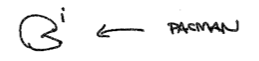
\includegraphics[width=.4\textwidth]{figures/lec05_pacman.png}
\end{center}
In this notation, the action of a basis dual vector on a basis vector is simply Pac-Man eating the basis vectors:
\begin{center}
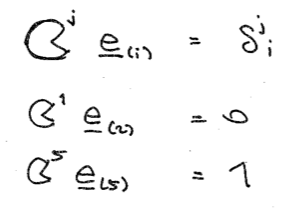
\includegraphics[width=.4\textwidth]{figures/lec05_paceats.png}
\end{center}
So we can write \eqref{eq:oneform:eats:vector} and \eqref{eq:oneform:eats:vector:basis} as
\begin{center}
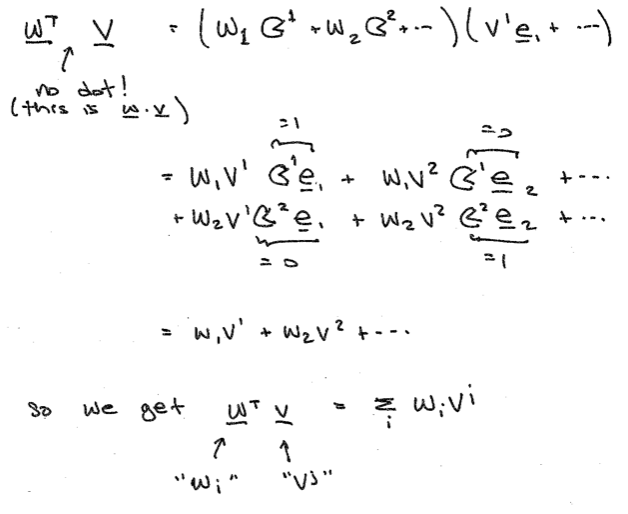
\includegraphics[width=.7\textwidth]{figures/lec05_paccontract.png}
\end{center}






\subsection{Orthonormal Bases}

At this point we should take a deep breath and state explicitly that we’ve been assuming an orthonormal basis. In this course we will continue to use an orthonormal basis. You may object to this and say that you used to believe in orthonormal bases until you were forced to write down the gradient (or worse, the Laplacian) in spherical coordinates. 
%
In other words, in principle one could imagine a basis where \eqref{eq:basis:dual:vec:act:on:vec} does not hold.
%
There are many things to be said about this, none of them are particularly edifying without a full discussion. With no apologies, I’ll make the following [perhaps perplexing] remarks:
\begin{enumerate}
\item There is no such thing as a `position vector.' Positions refer to some base space, whereas vectors (like differential operators) act on the tangent space at a point of that base space. 
\item A given tangent space is `nice’ and has a nice orthonormal basis. 
\item That basis may not be the same for neighboring tangent spaces (perhaps due to coordinates, perhaps due to intrinsic curvature). 
\end{enumerate}
In this course these nuances will not come up. In the rest of your life you’ll still have to deal with curvilinear coordinates. But suffice it to say that our study of function space will be nice an orthonormal. We haven’t yet given an adequate definition of `orthonormality,’ so let's take \eqref{eq:basis:dual:vec:act:on:vec} as a working definition.




\subsection{Bra-Ket Notation}

There is neither any physics nor mathematics contained in a choice of notation. However, a convenient notation does simplify our lives. Let us introduce bra-ket notation. In this notation, we denote vectors by kets:
\begin{align}
  |v\rangle = v^i|i\rangle \ ,
\end{align}
where $|i\rangle = \vec{e}_{(i)}$ is the basis of vectors that span the vector space $V$. There is nothing new or different about this object,  $\vec{v} = |v \rangle$.

We denote dual vectors (row-vectors, one-forms) as bras:
\begin{align}
  \langle w | &= w_i \langle i| \ ,
\end{align}
where $\langle i | = \tilde{\vec{e}}^{(i)}$. The orthonormality of this basis is encoded in 
\begin{align}
  \langle i | j \rangle = \delta^i_j \ .
\end{align}

In bra-ket notation a linear transformation $A$ has a basis
\begin{align}
  A = A^i_{\phantom{i}j} |i\rangle \langle j| \ .
\end{align}
The notation $|i\rangle \langle j|$ is shorthand for the \textbf{tensor product} $|i\rangle \otimes \langle j|$. If the $\otimes$ doesn’t mean anything to you, that’s fine. It doesn’t mean much to me either. Maybe you can replace it with the word `\emph{and}' so that $|i\rangle \otimes \langle j|$ means you have a basis ket $|i\rangle$ \emph{and} an basis bra $\langle j|$ that are somehow stuck together but aren't acting on each other. Matrix multiplication proceeds as before:
\begin{align}
  A\vec{v} = A|v\rangle = 
  A^i_{\phantom{i}j} |i\rangle \langle j| v^k |k \rangle
  = 
  A^i_{\phantom{i}j}  v^k  |i\rangle \langle j|k \rangle
  = 
  A^i_{\phantom{i}j}  v^k  |i\rangle \delta^j_k
  = 
  A^i_{\phantom{i}j}  v^j  |i\rangle \ .
\end{align}
Observe that the power of the notation is clear: the object with the index $v^i$ is just a number. It commutes with everything. All of the vector-ness is carried in the basis objects: the bras, kets, and ket-bras. Those do not commute. But they have a well defined way in which kets act on bras (or vice versa).\footnote{This is where the $\oplus$ notation is handy. It keeps track of which kets/bras might hit which other bras/kets. This falls under the name of multi-linear algebra.}


\subsection{Eigenvectors are nice}
\label{sec:eigenvectors}

Give a sufficiently \emph{nice} linear transformation, $A$, there is a particularly convenient basis: the eigenvectors of $A$. These are kets $|\lambda\rangle$ such that
\begin{align}
  A |\lambda\rangle = \lambda |\lambda\rangle \ .
\end{align}
In other words, $A$ acts on the eigenvector by rescaling. The rescaling coefficient is the eigenvalues. For \emph{nice} transformations (see Section~\ref{sec:niceness}), there is a complete set of such vectors to span the vector space.

If you write a general vector $|v\rangle$ in terms of this eigenbasis,
\begin{align}
  |v\rangle = v^i |\lambda_{(i)} \rangle \ ,
\end{align}
Then the action of $A$ on this vector is easy:
\begin{align}
  A |v\rangle = \sum_i \lambda_{(i)} v^i |\lambda_{(i)} \rangle \ .
\end{align}
In fact, assuming that all of the eigenvalues are non-zero, even the matrix inverse is easy:
\begin{align}
  A^{-1}|v\rangle = \sum_i \lambda_{(i)}^{-1} v^i |\lambda_{(i)} \rangle \ .
  \label{eq:linear:aglebra:inverse:eigenvectors}
\end{align}
The first time you see this should have brought a deep joy to your life: if you can decompose a matrix (linear transformation) into its eigenvectors and eigenvalues, then taking the inverse transformation is simple.


\subsection{Linearity of Inverse Operators}

Given a linear operator $A$, the inverse operator $A^{-1}$ is defined by
\begin{align}
  A^{-1} A = \mathbbm{1}_{N\times N} \ .
\end{align}
For an $N$-dimensional vector space, this represents $N^2$ different equations: one for each element. The inverse operator, by the way, is also linear. Let's remind ourselves of what this means. A linear transformation, when written as a matrix, is simply stating what that linear trasformation does to your basis vectors. If a matrix $B$ has elments
\begin{align}
  B = 
  \begin{pmatrix}
    a & b\\
    c & d
  \end{pmatrix}
  = 
  B^{i}_{\phantom{i}j} |i\rangle\langle j| \ , 
\end{align}
then this simply means that acting on basis vectors $\vec{e}_{(1)} = |1\rangle$ and $\vec{e}_{(2)} = |2\rangle$ gives
\begin{align}
  B|1\rangle &= a |1 \rangle + c|2\rangle 
  \\
  B|2\rangle &= b |1 \rangle + d|2\rangle  \ .
  \label{eq:B:basis:action}
\end{align}
In column vector notation:
\begin{align}
  B
  \begin{pmatrix}
  1 \\ 0
  \end{pmatrix}
  &= 
  \begin{pmatrix}
  a \\ c
  \end{pmatrix}
  &
  B
  \begin{pmatrix}
  0 \\ 1
  \end{pmatrix}
  &=
  \begin{pmatrix}
  b \\ d
  \end{pmatrix}\ .
\end{align}
So knowing the action on basis vectors is the same as knowing the transformation itself. Suppose I told you the action of the inverse transformation $A^{-1}$ on your basis vectors, vis-a-vis \eqref{eq:B:basis:action}:
\begin{align}
  A^{-1}|1\rangle &= x |1 \rangle + y|2\rangle 
  \\
  A^{-1}2\rangle &= z |1 \rangle + w|2\rangle  \ .
  \label{eq:Ainv:basis:action}
\end{align}
Then you know exactly how $A^{-1}$ acts on a general vector $|s\rangle = s^1|1\rangle + s^2 |2\rangle$:
\begin{align}
  A^{-1} |s\rangle &=
  A^{-1} \left( s^1|1\rangle + s^2 |2\rangle \right)
  \\ 
  &=
  s^1 A^{-1} |1\rangle + s^2 A^{-1} |2\rangle
  \label{eq:Ainv:basis:action:on:gen:step2}
  \\
  &=
  (s^1x + s^2z)|1\rangle + (s^1y + s^2 z)|2\rangle \ .
  \label{eq:Ainv:basis:action:on:gen}
\end{align}
You can now keep this in mind when we say we want to solve $A|\psi\rangle = |s\rangle$. If we knew the action of $A^{-1}$ on some basis of the space, then the problem is simple:
\begin{align}
  |\psi\rangle = \psi^i |i\rangle 
  &= \left( A^{-1} \right)^i_{\phantom{i}j} |i\rangle\langle j|
  \, s^k|k\rangle 
  \\
  &= \left(A^{-1}\right)^i_{\phantom{i}j} s^k \, |i\rangle\langle j|
  |k\rangle 
  \\
  &=\left(A^{-1}\right)^i_{\phantom{i}j} s^j \, |i\rangle \ .
\end{align}
We can write this as an equation for each component:
\begin{align}
  \psi^i &= \sum_j \left(A^{-1}\right)^i_{\phantom{i}j} s^j
  \label{eq:Ainv:acting:on:source} \ .
\end{align}
We've restored the explicit sum over $j$ as a convenient reminder. The quantity $\left(A^{-1}\right)^i_{\phantom{i}j}$ is what we would like to identify with a Green's function.







\subsection{The Green’s Function Problem}

Going back to the big picture: recall that we want to solve differential equations of the form $\mathcal O f(x) = s(x)$. If we had a sense of the \emph{eigenfunctions} of $\mathcal O$, then we could expand $s(x)$ in a basis of those eigenfunctions and then apply $\mathcal O^{-1}$ to both sides. 

The analog is this:

\begin{center}
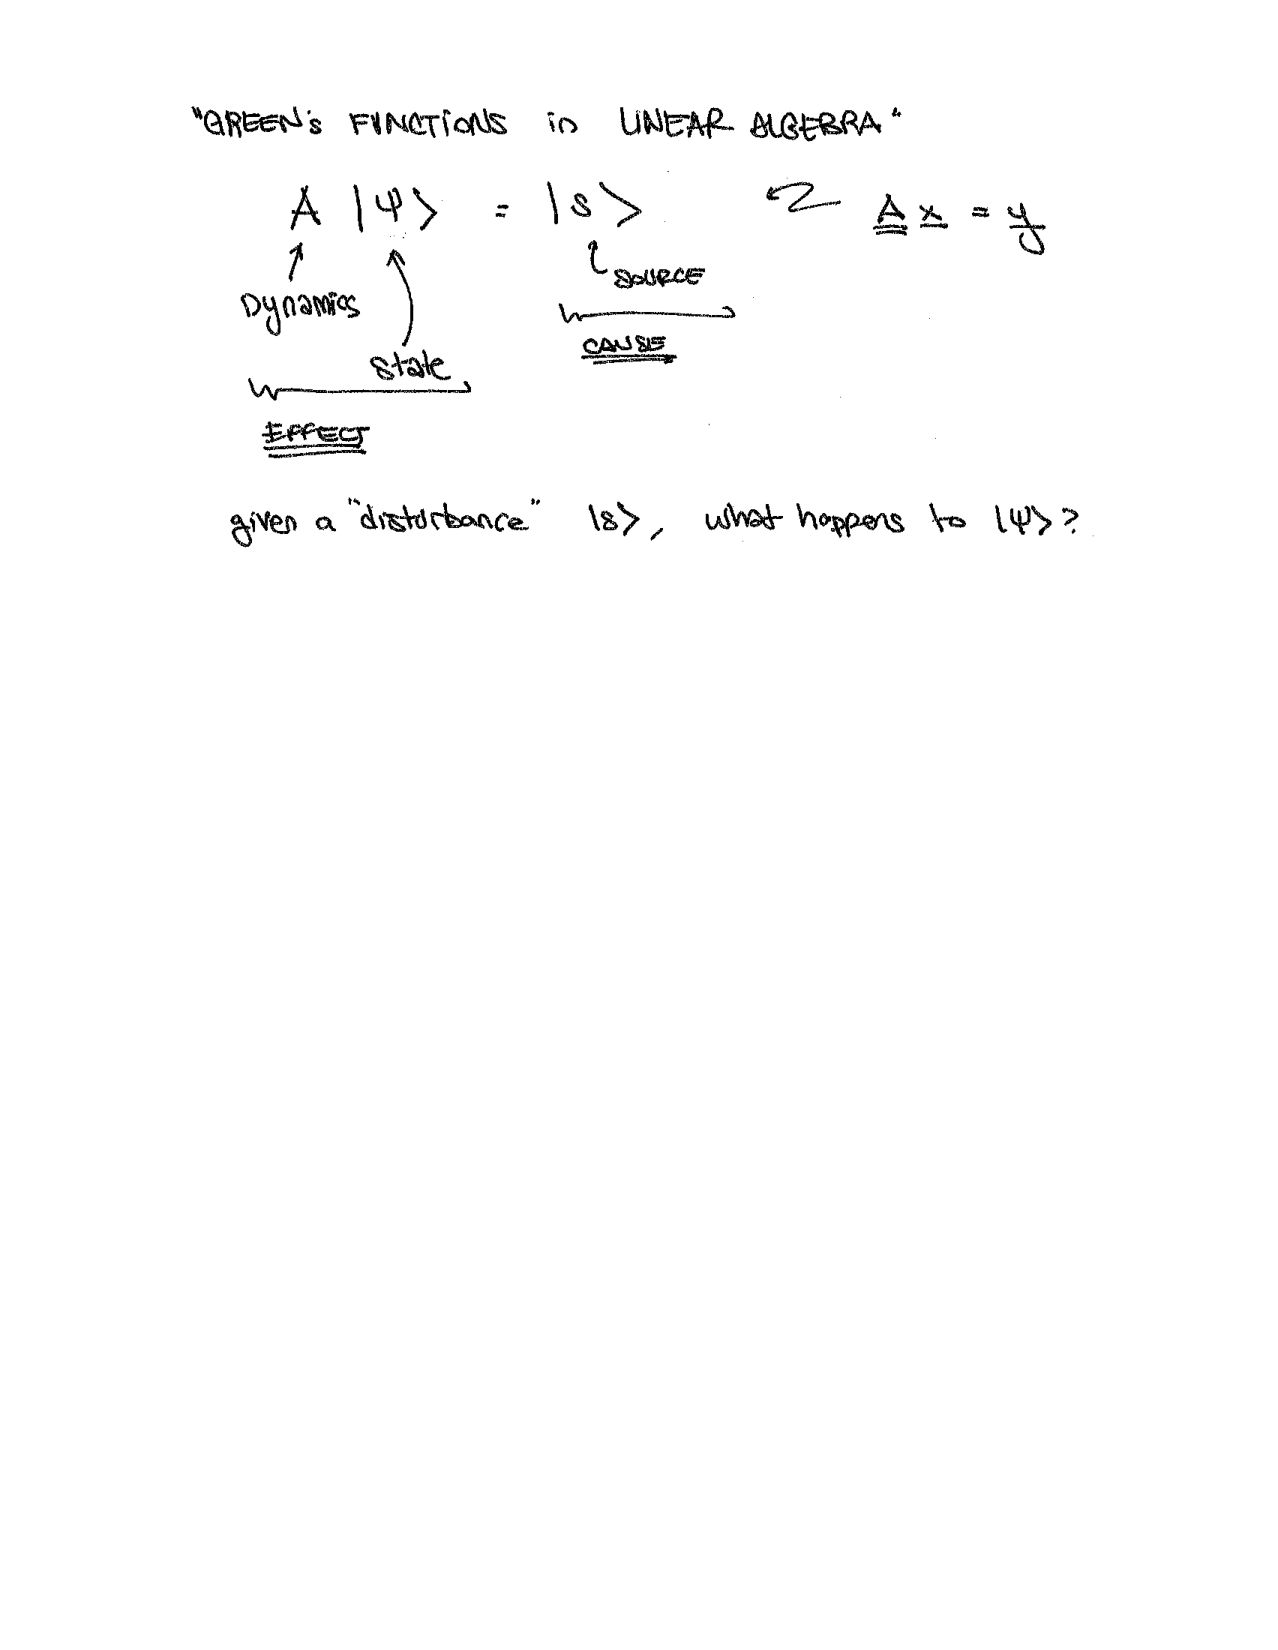
\includegraphics[width=.7\textwidth]{figures/lec02_green01.pdf}
\end{center}

 The operator $A$ encodes the \emph{physics} of the system, the underlying dynamics. This is presumably local: it is a near-diagonal matrix coming from one or two powers of derivatives.  The ket $|s\rangle$ is the source. This is the thing that \emph{causes} the dynamics. The ket $|\psi\rangle$ is some state that we would like to determine. \eqref{eq:linear:aglebra:inverse:eigenvectors} is telling us that to invert a differential operator $\mathcal O$, it may be useful to decompose it into \textbf{eigenfunctions}.

 By the way, \emph{this} is where all of the `special functions' in your physics education show up. The reason why you would ever care about Bessel functions (of various kinds) or Legendre polynomials is simply that they are the eigenfunctions of differential operators that we care about\footnote{In fact, they're mostly the eigenfunctions of the same differential operator in different coordinate systems. Do you know which differential operator? I'll give you a guess. It's starts with a `har-' and ends with a `monic oscillator.'}. Sometimes we confuse mathematical physics with `properties of special functions.' I do not care about special functions; perhaps with the notable exception of the $\Gamma$-function. Seriously, to screw special functions. The real intuition for what we're doing is evident in the few-dimensional harmonic oscillator. All the Bessel-schmessel function-ology that will pain you in your Jackson E\&M course are just \emph{technical details}.

\begin{example}
Consider a differential operator $A\to \mathcal O = (d/dx)^2$. There's a basis of nice eigenvectors $\xi_{(k)}$:
 \begin{align}
   \xi_{(k)} &= \sin (kx)
   &
   \mathcal O \xi_{(k)} &= -k^2 \xi_{(k)}. 
 \end{align}
 I've deliberately avoided normalizing for now. From this you can see that writing a function as a \textbf{Fourier Series} is simply a change of basis to eigenfunctions of $(d/dx)^2$. Can you see how you would `invert' this operator acting on a general function $f(x)$ with a set of Fourier coefficients $f(x) = \sum_k c_k\sin(kx)$?
\end{example} 


\begin{example}\label{eq:charged:cat}
A common example in electrostatics is the triboelectric effect. Go ahead, take a moment to look it up on Wikipedia. The image is very relevant. If you pet your cat with hard rubber\footnote{I do not recommend doing this.}, the cat builds up some electrostatic charge. For simplicity, let's model this system as a bunch of Lego blocks arranged in a cat-shape where each block has a constant electric charge. Let's say that each block has volume $dV$ and constant charge density $\rho_0$ so that each block has charge $\rho_0 dV$. The entire cat is described by a charge density $\rho(x)$ where $\rho(x)=0$ if you're outside the cat and $\rho(x)=\rho_0$ if you're inside the cat. 
\begin{center}
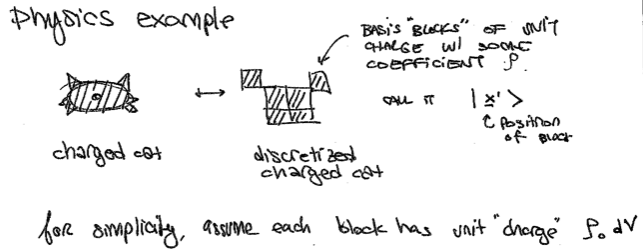
\includegraphics[width=.8\textwidth]{figures/lec06_cat.png}
\end{center}
You know how this problem works. You want to solve for the electrostatic potential, $\Phi(x)$, given the charge density $\rho(x)$. The relevant equation is
\begin{align}
  \nabla^2 \Phi(\vec{x}) = -\rho(\vec{x})\ ,
\end{align}
where $\epsilon_0=1$ in convenient units. This looks like a tricky differential equation to solve, but the fist week of our undergraduate electrodynamics course taught us that the potential from a \emph{unit point charge} is
\begin{align}
  \Phi(\vec{x}) = \frac{-1}{4\pi} \frac{1}{|\vec{x}-\vec{x}'|} \ .
\end{align}
The relevant diagram is
\begin{center}
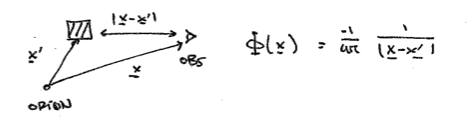
\includegraphics[width=.6\textwidth]{figures/lec06_1charge.png}
\end{center}
If we know the potential from a single point charge, then we can invoke linearity---specifically, the linearity of $\nabla^2$)---to write down the potential for two unit point charges: 
\begin{center}
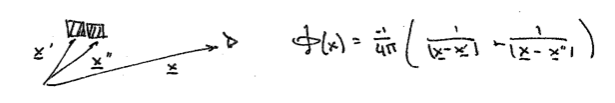
\includegraphics[width=.7\textwidth]{figures/lec06_2charge.png}
\end{center}
At this point, you should start to see how this looks just like \eqref{eq:Ainv:basis:action:on:gen}. The result is
\begin{align}
  \Phi(\vec{x}) &= 
  \sum_{\vec{x}'} \frac{-1}{4\pi} \frac{1}{|\vec{x}-\vec{x}'|} \rho(\vec{x}') dV
  \;\to \;
 \int d^3\vec{x}' \frac{-1}{4\pi} \frac{1}{|\vec{x}-\vec{x}'|} \rho(\vec{x}')   \ .
 \label{eq:electrostatics:greens:func}
\end{align}
\end{example}
This last example is really useful. You've seen this calculation before, but please review it carefully from the perspective of the action of $(\nabla^2)^{-1}$. Just as we are able to build a `Lego cat' out of unit blocks, each of those unit blocks comes with an electrostatic potential. The solution to $\nabla^2 \Phi(x) = -\rho(x)$ is to simply sum together those point-source solutions in the same way that one sums together the point sources (assembles the blocks) to model the finite source.

\begin{exercise}
In the example above, what plays the role of the basis vectors? 
\end{exercise}

Compare \eqref{eq:electrostatics:greens:func} to \eqref{eq:Ainv:acting:on:source}. The sum over positions $\vec{x}'$ that becomes an integral over $d^3\vec{x}'$ is completely analogous to the sum over the index $j$. $\rho(\vec{x}')$ plays the role of a component of the source, $s^j$. On the left-hand side, $\Phi(\vec{x})$ plays the role of $\psi^i$. We note that the index $i$ is replaced by the position $\vec{x}$. Evidently, the inverse of $\nabla^2$ is simply
\begin{align}
  (\nabla^2)^{-1} \equiv G(\vec{x},\vec{x}') = -\frac{1}{4\pi} \frac{1}{|\vec{x}-\vec{x}'|} \ .
  \label{eq:laplacian:greens:func:eg}
\end{align}
Here we've written out $G(\vec{x},\vec{x}')$, the Green's function for $\nabla^2$. Observe that the Green's function has two arguments in the same way that the inverse matrix $\left(A^{-1}\right)^i_{\phantom{i}j}$ has two indices. The $\vec{x}'$ `index' is integrated/summed over---it scans each `building block' of the source in the same way that we sum over $j$ in the index contraction $\left(A^{-1}\right)^i_{\phantom{i}j}s^j$. In other words, we may heuristically write \eqref{eq:laplacian:greens:func:eg} as
\begin{align}
  \Phi^i \sim \sum_j G^i_{\phantom{i}j}\rho^j \ .
\end{align}

At this point, it's useful to point out that the Green's function is often called a \textbf{propagator}. As a function, $G(x,x')$ propagates the information of the source at $x'$ to the observer at $x$ assuming some dynamics---the operator for which $G$ is a Green's function.
\begin{center}
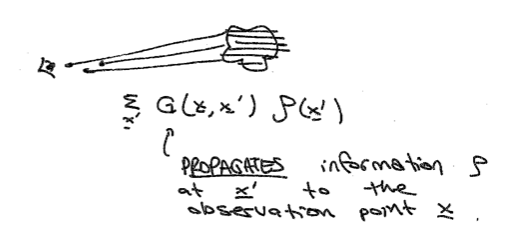
\includegraphics[width=.5\textwidth]{figures/lec06_propagator.png}
\end{center}

Please, please, please make sure you understand this example. This will be the key starting point from which we will generalize our study of Green's functions in physics.

\subsection{Remark: Implicit assumption of linearity}

In everything we're building we're assuming that the dynamics that relates  the source $|s\rangle$ and the state $|\psi\rangle$ is \emph{linear}. That's why we can think of the differential operator $\mathcal O$ as a matrix. If $|\psi_0$ is the effect of source $|s_0\rangle$, then you know by linearity that $2|\psi_0\rangle$ is the effect of a source that is twice as strong, $2|s_0\rangle$. 

Linearity is \emph{not} a truth of nature, yet we're spending all of this course developing techniques for dealing with linear dynamics! The fact of the matter is that a good chunk of physics \emph{is} linear---and that's good because those are the parts that we can solve using our standard toolkit. Most of the frontier of physics has to do with how to deal with the \emph{non}-linearities. There are a few options here: numerical solution, perturbation expansions about a linear solution (Feynman diagrams), and looking for topological invariants. 





\subsection{Metrics on Finite Dimensional Vector Spaces}

Thus far we have introduced vector spaces. The dual vector space is a set of linear functions that act on elements of a vector space; these are bras/row-vectors/one-forms. Let us now introduce a new piece of machinery: a \textbf{metric}. This is also known as an \textbf{inner product} or a \textbf{dot product}. A space with a metric is called a metric space. We only state this fact to emphasize that we are \emph{adding this structure by hand}. Vector spaces don't come with metrics---someone makes up a metric and slaps it onto the vector space.

The \textbf{metric} is a function that takes two vectors and spits out a number. It is linear in each argument. In other words, a metric $g$ is:
\begin{align}
  g:\; V\times V\to \mathbb{R} \ .
\end{align}
Occasionally one may want a metric defined such that the output is a complex number. We thus have:
\begin{align}
  g(\alpha \vec{v} + \beta\vec{w}, \delta \vec{x} + \gamma \vec{y})
  &= 
  \alpha \delta g(\vec{v},\vec{x}) + \alpha \gamma g(\vec{v},\vec{y}) + \beta\delta g(\vec{w},\vec{x}) + \beta\gamma g(\vec{w},\vec{y}) \ .
\end{align}
One more special assumption about the metric is that it is \textbf{symmetric}\footnote{Actually it is conjugate symmetric, $g(\vec{v}, \vec{w}) = g(\vec w, \vec v)^*$. This distinction will be important for function spaces.}:
\begin{align}
  g(\vec{v},\vec{w}) = g(\vec{w}, \vec{v}) \ .
\end{align}
In indices one may write
\begin{align}
  g &= g_{ij} \langle i | \otimes \langle j |
\end{align}
so that
\begin{align}
  g(\vec{v}, \vec{w}) = g_{ij} v^{i}w^j \ .
 \end{align}
 Here we see the usefulness of the $\otimes$ notation. It tells us that the bras and kets resolve as follows:
 \begin{align}
   g_{ij}\langle i | \otimes \langle j | \left(v^k|k\rangle\right)\left(w^\ell|\ell\rangle\right) 
   = 
   g_ij v^k w^\ell 
   \langle i | k\rangle \langle j |\ell\rangle
   = 
   g_ij v^k w^\ell  \delta^i_k \delta^j_\ell 
   = 
   g_{ij} v^{i}w^j \ .
   \label{eq:metric:basis:vectors}
 \end{align}
 If this is your first time seeing it, please re-read \eqref{eq:metric:basis:vectors} carefully to see exactly how the bras and kets resolve themselves. 
 %
 For ordinary Euclidean space in flat coordinates, the metric is simply the unit matrix: $g_{ij} = \text{diag}(1,\cdots, 1)$. In Minkowksi space there’s a relative minus sign between space and time. In curvilinear coordinates things get ugly. 
 
Here’s the neat thing about metrics. We can take a metric $g$ and pre-load it with a vector $\vec{v}$: 
\begin{align}
  g(\vec v,\qquad ) \ .
\end{align}
In fact, we may then define a function with respect to this pre-loaded metric:
\begin{align}
  f(\vec{w}) = g(\vec v,\vec w)
\end{align}
Observe that $f(\vec{w})$ is a linear function that takes elements of $V$ and returns a number. In other words, this is a \emph{dual vector} (row-vector, one-form, element of $V^*$). The metric has allowed us to \emph{convert vectors into dual vectors}:
\begin{align}
  g(\vec v,\qquad )  = g_{ij} v^i \langle j| \ .
  \label{sec:ket:as:pre:loaded:metric}
\end{align}

Similarly, one may define an inverse metric $g^{-1}$ such that $g^{-1}g = \mathbbm{1}$. In a slight abuse of notation, the inverse metric is written with two upper indices: $g^{ij}$. Note that we do not write the `$^{-1}$.' The inverse metric will \emph{raise} the index on a lower-index object, while the metric \emph{lowers} the index of an upper-index object.\footnote{Of course: what’s really happening is that the metric has a basis $\langle i|\otimes \langle j|$ while the inverse metric has a basis $|i\rangle \otimes |j\rangle$.}


\subsection{The dot/inner product, orthonormality}

You are already familiar with the `obvious' way to take two vectors and spit out a number. This is the dot product of two vectors, also known as the inner product. They are equivalent to each other and equivalent to the action of the metric on a pair of vectors;
\begin{align}
  \vec v\cdot \vec w = \langle \vec v, \vec w \rangle = g(\vec v, \vec w) \ .
\end{align}
The norm of a vector $\vec v$ is simply the square root of $g(\vec v, \vec v)$. 
%
By the linearity of the metric, we can decompose the dot product into the action of the metric on basis vectors:
\begin{align}
  g(\vec v, \vec w) &= 
  g(
    v^1\vec e_{(1)} + v^2\vec e_{(2)} + \cdots,
    w^1\vec e_{(1)} + w^2\vec e_{(2)} + \cdots
  )
  \\
  &=
  v^1 w^1 g(\vec e_{(1)}, \vec e_{(1)}) + 
  v^1 w^2 g(\vec e_{(1)}, \vec e_{(2)}) + \cdots \ ,
\end{align}
where our assumption of an \emph{orthonormal basis}\footnote{Not an `oprhan normal' basis like Zoom's auto-transcription claims I said.} is the statement that
\begin{align}
  g(\vec e_{(i)}, \vec e_{(j)}) = \pm \delta^i_j \ .
  \label{eq:orthonormal}
\end{align}
The $\pm$ depends on the signature of the metric. As physicists, this is the distinction between `space' and `time.' For Euclidean space the sign is always plus. For Minkowski spacetime, there's some choice of sign for the timelike direction and the opposite sign for the spacelike direction. The choice is a convention, there's no `right' choice\footnote{The right choice is $+$ for timelike and $-$ for spacelike.}. When \eqref{eq:orthonormal} is not true the basis is not orthonormal. Sometimes this happens when your space is curvy (general relativity); other times you just have curvilinear coordinates for a flat space (e.g.~polar coordinates). I'm glossing over several subtleties here, among them is the idea that position vectors do not exist\footnote{Formally, vectors live in the tangent space of a manifold. They are `intrinsically' tangent vectors (velocities) of some trajectory on the manifold with some `time' parameter. The position on the manifold is a coordinate, but it is not a \emph{vector}. For more on what I mean by this, I recommend \texttt{hep-th/0611201}, Arnold's \emph{Mathematical Methods of Classical Mechanics}, or a graduate general relativity textbook.}.
\begin{exercise}
Speaking of the notion of curved space: Consider a sheet of paper as an idealized two-dimensional surface. If you tape opposite edges of the paper together to make a cylinder, is the two-dimensional space curved or flat? For example, if two-dimensional beings lived on the paper like in Edwin Abbot--Abbot's novella \emph{Flatland}, would they say that their space is curved? 
\end{exercise}
\begin{exercise}
The cylinder from the previous exercise is an example of periodic boundary conditions. For those familiar with special relativity, this entire section has probably been a big review. Here's a fun puzzle to think about while you skim. What happens to the twin paradox if the universe were periodic in some spatial direction? The usual resolution to the twin paradox is that the twin that `turns around' must change inertial frame. However, if there were a periodic direction, neither twin has to `turn around' for them to meet once again and compare clocks\footnote{For a nice solution, see: \url{https://doi.org/10.1080/00029890.2001.11919789}}.
\end{exercise}
\begin{example}\label{eg:two:ways:to:contract}
Given two vectors $\vec v$ and $\vec w$, there are two equivalent ways of thinking about how they may be combined into a number. First, one can lower the index of one of the vectors with the metric $v_i \equiv g_{ij}v^i$ and then contract the `row vector' $v_i$ with the `column vector' $w^j$: $v_iw^i$. I am of course abusing notation by conflating the components $v_i$ and $w^j$ with the row/column vectors. The second way of doing this is taking the two vectors and contracting them directly with the metric: $v^i w^j g_{ij}$. Please make sure you are comfortable that these `two ways' are exactly the same thing.
\end{example}

\subsection{Comment: Why physicists like indices}

Einstein's summation convention tells us that we should see repeated upper/lower indices as contracted pairs---we should treat them differently. In contrast, the un-paired indices tell us something about the physical quantity to which those indices are attached. This is why---despite what our mathematician colleagues tell us---we love indices\footnote{Recent Nobel laureate Roger Penrose has a clever notation that replaces indices with lines; \url{https://en.wikipedia.org/wiki/Penrose_graphical_notation}.} Vectors are objects that transform in a well defined way with respect to rotations: $$v^i \to v'^i = R^i_{\phantom{i}j}v^j \ , $$ where $R$ is a rotation matrix. Similarly, one-forms/column vectors transform `oppositely': 
\begin{align}
  w_k \to w'_k = \left(R^T\right)^\ell_{\phantom{\ell}k}w_\ell \ .
\end{align}
Observe that the rotation matrix is \emph{transposed} when acting on an \emph{lower} index object.
%
This is consistent with the idea that the dot product is invariant under rotations:
\begin{align}
  v^i w_i 
  \to 
  v'^i w'_i 
  =R^i_{\phantom{i}j}v^j \left(R^T\right)^\ell_{\phantom{\ell}i}w_\ell
  = \left[\left(R^T\right)^\ell_{\phantom{\ell}i} R^i_{\phantom{i}j}\right] v^j w_\ell
  = v^j w_j \ ,
  \label{eq:moving:terms}
\end{align}
where we've used the fact that the matrix in the square brackets is simply $\delta^\ell_j$ which is evident from $R^TR = \mathbbm{1}$.
\begin{example}
We exploited something neat about the index notation in \eqref{eq:moving:terms}. Note that there aren't any `vectorial' objects in \eqref{eq:moving:terms}---all there is are a bunch of numbers (components of vectorial objects). We used the fact that we could re-arrange these products to make it clear how they contract. That's why we were able to move the $(R^T)^\ell_{\phantom{\ell}i}$ term all the way to the left. 
\end{example}
A neat lesson here is that
\begin{quote}
Indices tell us how an object transforms under `rotations'.
\end{quote}
Here `rotations' mean whatever the appropriate symmetry is. In quantum mechanics, for example, the rotations are unitary transformations. If an object has indices, then it transforms. If an object has no indices (or is only composed of contracted indices) then it is a scalar with respect to those transformations. 
%
This `indexology' is the backbone of how lazy physicists apply representations of symmetry groups\footnote{\url{https://github.com/Tanedo/Physics262-2019}}. It's especially useful in particle physics\footnote{\url{https://sites.google.com/ucr.edu/p165/}}.

The generalization to tensors is hopefully clear. An object with some number of upper indices and some number of lower indices transforms with several factors of the rotation matrix and its transpose:
\begin{align}
  T^{i_1i_2\cdots i_n}_{\phantom{i_1i_2\cdots i_n}j_1j_2\cdots j_m}
  \to 
  R^{i_1}_{\phantom{i_1}k_1}R^{i_2}_{\phantom{i_2}k_2}\cdots R^{i_n}_{\phantom{i_n}k_n}
  (R^T)^{\ell_1}_{\phantom{\ell_1}j_1}
  (R^T)^{\ell_2}_{\phantom{\ell_2}j_2}
  \cdots
  (R^T)^{\ell_m}_{\phantom{\ell_m}j_m}
  T^{k_1k_2\cdots k_n}_{\phantom{k_1k_2\cdots k_n}\ell_1\ell_2\cdots \ell_m} \ .
\end{align}
Yes, we are so wealthy with indices that our indices have indices.
\begin{exercise}
How does the moment of inertia tensor transform under a rotation $R$?
\end{exercise}

\subsection{Adjoints and Hermitian Conjugates}
% Lec09.pdf of 2018 notes
% with 4.4 of Byron and Fuller

Because the metric lowers the index of a vector and produces a dual vector, you may want to think about this as `tipping over' a column vector---almost like a transpose, right? We should be careful with this notion. Suppose we have a vector $\vec{w} = A \vec{v}$. How do we express the components of the \emph{dual vector} $w_i$ with respect to the elements of the dual vector $v_i$?
\begin{align}
  w_i = g_{ij}w^j
  = g_{ij}\mat{A}{j}{k} v^k
  = A_{jk}v^k
  = A_{j}^{\phantom{j}k}v_k
  \equiv 
  v_k \mat{(A^T)}{k}{j}
  \ . \label{eq:wi:and:transpose:A}
\end{align}
In the second-to-last step we have used $g^{ij}g_{jk} = \delta^i_k$. In the last step we have \emph{defined} the transpose of a real matrix in the usual way: swap the first and second indices. These happen to have heights that come along for the ride. For convenience we moved the $v_k$ to the left-side of the expression---it should be clear that this does not affect the expression at all (just write out the sum explicitly). We've gone through these gymnastics simply to motivate the notion that
\begin{align}
  \vec{w}^T = \vec{v}^T A^T \ .
\end{align}
Notice that the $T$ \emph{acts} on the matrix $A$. This is in contrast to our notation where the $T$ in $\vec{w}^T$ is simply a label to remind us that the object is a dual (row) vector.


For complex vector spaces---for example, the space of wavefunctions in quantum mechanics---we need to be a little bit more careful. We won't say much about complex vector spaces in general, but us simply state that the `transpose’ is generalized to the Hermitian conjugate. You may be most familiar with this in bra-ket notation from quantum mechanics:
\begin{align}
  \langle x| = |x\rangle^\dag = \langle x, \quad \rangle \ ,
\end{align}
where $\langle x, \quad \rangle$ is simply the inner product on the complex space with one component pre-loaded\footnote{By the way, this motivates the bra-ket notation for vectors and dual-vectors:
\begin{align}
  \langle x | y\rangle  = \langle x, y\rangle \ .
\end{align}
In the above equation, the left-hand side is a bra (dual vector) acting on a ket (vector), while the right-hand side is the inner product acting on two kets. This is simply repeating the statement in Example~\ref{eg:two:ways:to:contract}. }. You should now see why the Hermitian conjugate isn't just a `transpose' but also a complex conjugation. The \textbf{norm} of a vector is $||\vec v || = \langle \vec{v},\vec{v}\rangle$. We would like the \textbf{norm} to be positive definite\footnote{The notable exception is when you have a space with nontrivial signature like Minkowski space where the relative sign between space and time is relevant.}, even when $\vec v$ is complex. If $\vec v$ has a complex phase, then there needs to be a `complex conjugation' built into the notion of an inner product. 
\begin{example}
While this may sound like hand-waving, you already know this from quantum mechanics where the wavefunction $\psi(x)$ is complex. You know that a nice wavefunction is normalized, $\langle \psi,\psi\rangle = 1$, which we interpret as:
\begin{align}
  \int dx\, \psi^*(x)\psi(x) = 1 \ .
\end{align}
The $\psi^*(x)$ in the integrand is related to the complex conjugation implicit when going from a ket $|\psi\rangle$ to a bra $\langle \psi|$. 
\end{example}
We will work this out more carefully when we re-introduce function spaces systematically---but all of this should feel familiar. 

Let us write \textbf{adjoint} to mean transpose for real spaces and Hermitian conjugate for complex spaces. The importance of the adjoint is not converting vectors into dual vectors, but rather the action on operators. Armed with a metric/inner product, the adjoint $A^\dag$ of an operator $A$ satisfies
\begin{align}
  \langle A^\dag w, v  \rangle
  = 
  \langle w, Av \rangle \ .
  \label{eq:adjoint:definition}
\end{align}
In a given inner product, the adjoint shifts the action from one vector to the other. 
\begin{example}
From this definition, it should be clear that
\begin{align}
  \langle w |  A v\rangle = \langle A^\dag w | v\rangle \ .
  \label{eq:wAv:Awv}
\end{align}
This equation does not invoke the metric in contrast to \eqref{eq:adjoint:definition}. Of course, the dual vector $\langle w |$ is related to the vector $|w\rangle$ by the metric.
\end{example}
\begin{exercise}
If you are mathematically inclined, prove the existence, uniqueness, and linearity of the adjoint $A^\dag$ of a linear operator $A$. \emph{Hint: see Byron \& Fuller chapter 4.4}. 
\end{exercise}

The adjoint/Hermitian conjugate is important because of the result that \textbf{self-adjoint operators}, $A^\dag = A$, have real eigenvalues and a complete set of orthogonal eigenvectors. Then we can use the strategy of Section~\ref{sec:eigenvectors} to use eigenvectors of $A$ to simplify the solution of $A\vec{v} = \vec{w}$.